   \documentclass[preprint,1p,times]{elsarticle}
 
 \usepackage{graphicx}
 %% The amssymb package provides various useful mathematical symbols
 \usepackage{amssymb} 
 \usepackage{lineno}
 
 
 \usepackage{amsmath}
 \usepackage{siunitx}
 \usepackage{tabularx}
 %\usepackage{algorithm2e}
 %\usepackage{algorithm,algorithmicx}
 \usepackage{amsmath,algpseudocode}\usepackage{algcompatible}
 \usepackage{amsthm}
 \usepackage{graphicx}
 \usepackage{lscape}
 \usepackage{verbatim}
 \usepackage{color,soul}
 \usepackage{xcolor}
 \usepackage{subfigure}
 \usepackage{tabularx,ragged2e,booktabs,caption,array,multirow,multicol}
 \usepackage{hyperref}
 \usepackage{csquotes}
 \usepackage{mathtools} 
 \usepackage{amsthm}  
 \usepackage{listings}
 \usepackage{amssymb}
 \usepackage{latexsym}
 \usepackage{epsfig}
 \usepackage{float}
 \usepackage{xspace}
 %\usepackage{algorithmwh}
 \usepackage{float}

 \newcommand\eindent{\endgroup}
 \newcommand{\mb}[1]{\mathbf{#1}}
  \newcommand{\bs}[1]{\boldsymbol{#1}}
  \newcommand{\mc}[1]{\mathcal{#1}}% \usepackage{varwidth}


 %\journal{IEEE Tran. Geo. Remote Sens.}

 \begin{document}

 % \begin{frontmatter}
 %
 % %% Title, authors and addresses
 %
 % \title{Bayesian inference via multi-core parallel tempering approach for  basin and landscape  evolution}
 %
 % \author[ctds,grg]{Rohitash Chandra\corref{cor2}}
 % \ead{rohitash.chandra@sydney.edu.au}
 % \author[grd,sih]{R. Dietmar M\"uller}
 % \author[ctds]{Ratneel Deo}
 % \author[sih]{Nathaniel Butterworth}
 % \author[grg]{Tristan Salles}
 %
 % \author[ctds,math]{Sally Cripps}
 % \address[grg]{EarthByte Group, School of Geosciences, University of
 % Sydney, NSW 2006, Sydney, Australia}
 % \address[ctds]{Centre for Translational Data Science, University
 % of Sydney, NSW 2006, Sydney, Australia}
 %
 % \address[sih]{Sydney Informatics Hub, University
 % of Sydney, NSW 2006, Sydney, Australia}
 %
 %
 % \address[math]{School of Mathematics and Statistics, University
 % of Sydney, NSW 2006\\Sydney, Australia}
 %
 % \end{frontmatter}
  %-----------------------------------
   %-----------------------------------
 
\section{Computational environment for Parallel Tempering Bayeslands Experiments}
All parallel tempering Bayeslands simulations were run on The University of Sydney HPC, Artemis. We utilised nodes built from Dell EMC Powedge C6420, with 48 cores and 192 GB per node. Our parallel tempering algorithm cannot communicate accross nodes so were run on a maximum of 48 cores. The design of the algorithm means it will only be as fast as it's slowest chain, so we see a plateau in speed improvement after around 20 replicas/cpus. As each node has 48 cores, we chose to run our primary experiments on 24 cores to fit within the node. RAM usage fluctuates depending on experiment, number of samples, replicas, etc, but is on the order of 2--60\,GB. Model variables were systematically explored to determine optimal and robust parameter choices for each experiment. The full set of successful experiments can be found in the accompaning spreadsheet \textit{BayeslandsRuns.xlsx}.

\section{Expanded results}
Summary of results for each problem, with optimal model parameters, replicated from the main paper, is shown here in Figrue \ref{tab:all_res}. The optimal model parameters, based on a balance of computational time and experimental accuracy accross all four problems, were drawn from the complete set of experiments. Several of the insights, and the evolution of the models, for these results are shown in Figures \ref{fig:crater_fast_cross}--\ref{fig:pos_allprob}. 
 
 \begin{table*}[htbp!]
 \centering
 \small
  \begin{tabular}{ l c c c c c} 
  \hline\hline
 Topography & Time (minutes) & Sed. RMSE &  Elev. RMSE   & Pred. RMSE & Accepted \%  \\  
  \hline\hline
 Crater-short & 	102	& 4.3	& 	1.1 &   5.4 & 19.17 \\
 Crater & 	275	& 0.9	& 1.3  	&  2.2 & 8.56 \\
 Etopo-short & 	68	& 60.0	& 587.9	&   11.0 &  4.62 \\
 Etopo &	325	& 55.3	& 46.1 &    101.4	 & 1.42 \\
  \hline
  \end{tabular}
 
 \caption{Results for respective problems (24 replicas/cores and 100\,000 samples). }
  \label{tab:all_res} 
 \end{table*}
 

 %----------------------------------
 % CRATER SHORT
  %-----------------------------------

  \begin{figure*}[htb!]
{\centering
      \begin{tabular}{cc}
        \subfigure[Elevation cross-section along x-axis]{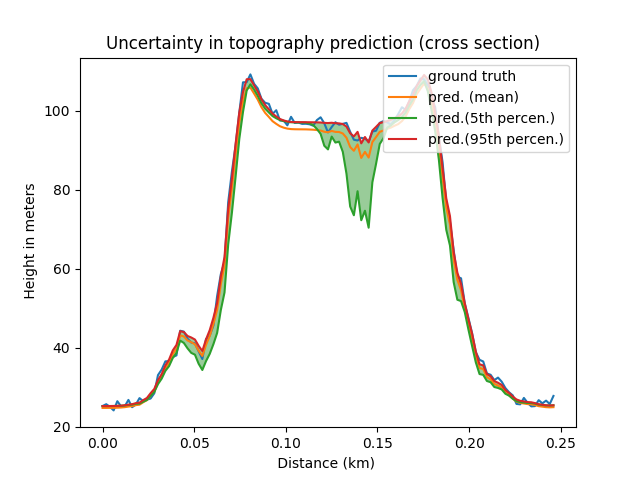
\includegraphics[width=70mm]{crater_fast/x_ymid_opt.png}}
        \subfigure[Elevation cross-section along y-axis]{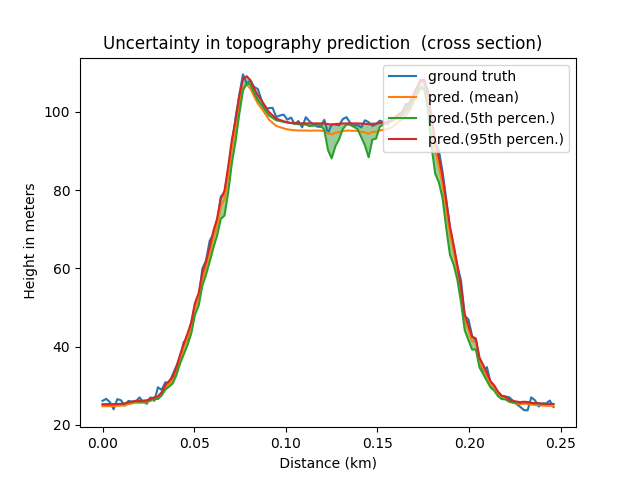
\includegraphics[width=70mm]{crater_fast/y_xmid_opt.png}}\\
      \end{tabular}
      \caption{Crater-short: Elevation cross-section taken at mid-point along x-axis and y-axis }
   \label{fig:crater_fast_cross}
}
  \end{figure*}


  %-----------------------------------

 \begin{figure*}[htb!]
{
\centering
     \begin{tabular}{cc}
       \subfigure[Crater-short erosion-deposition after 25 \% evolution time ]{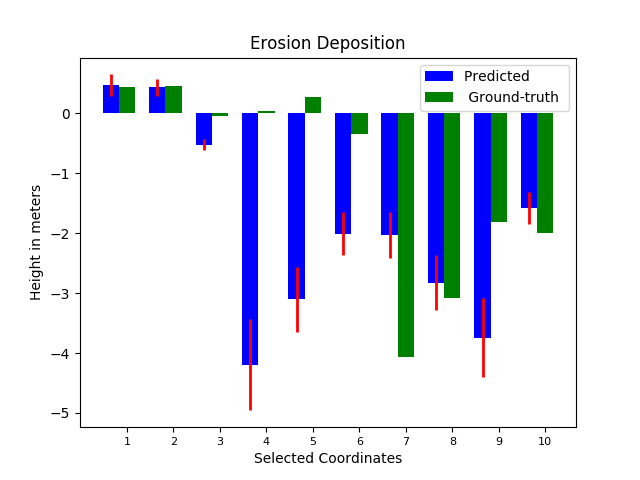
\includegraphics[width=80mm]{crater_fast/pos_erodep_3750.png}}
       \subfigure[Crater-short erosion-deposition  after 50 \% evolution time]{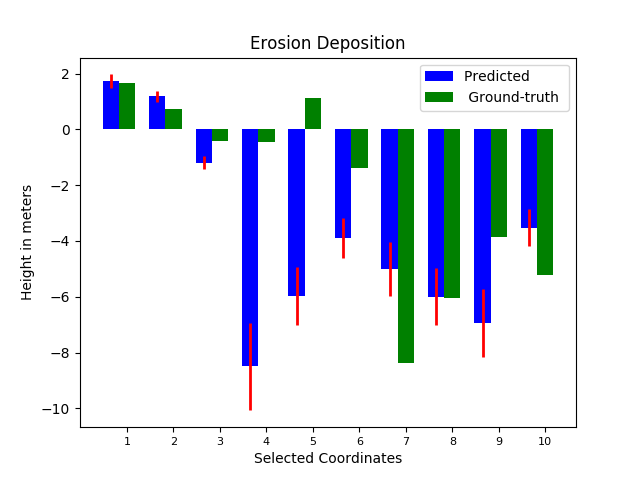
\includegraphics[width=80mm]{crater_fast/pos_erodep_7500.png}}\\
        \subfigure[Crater-short erosion-deposition after 75 \% evolution time ]{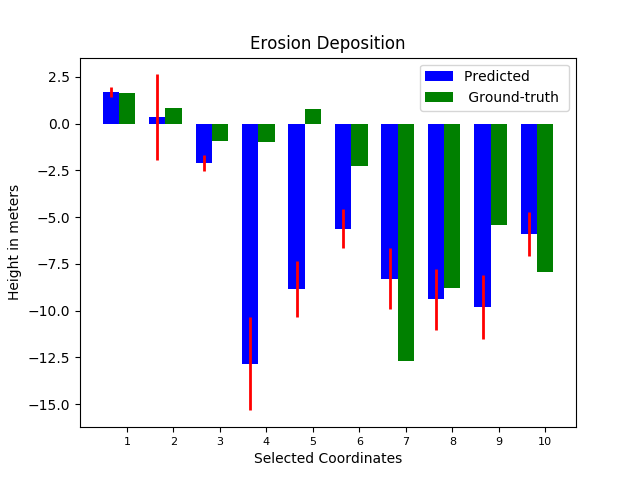
\includegraphics[width=80mm]{crater_fast/pos_erodep_11250.png}}
       \subfigure[Crater-short erosion-deposition  after 100 \% evolution time]{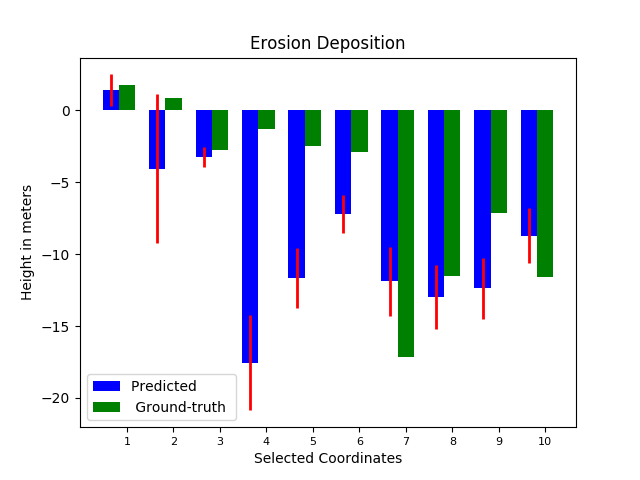
\includegraphics[width=80mm]{crater_fast/pos_erodep_15000.png}}\\
     \end{tabular}
     \caption{Crater-short erosion-deposition   }
  \label{fig:crater_fast_erodep}
}
 \end{figure*}


 %----------------------------------

 \begin{figure*}[htb!]
{
\centering
     \begin{tabular}{cc}
       \subfigure[Crater-short rainfall distribution]{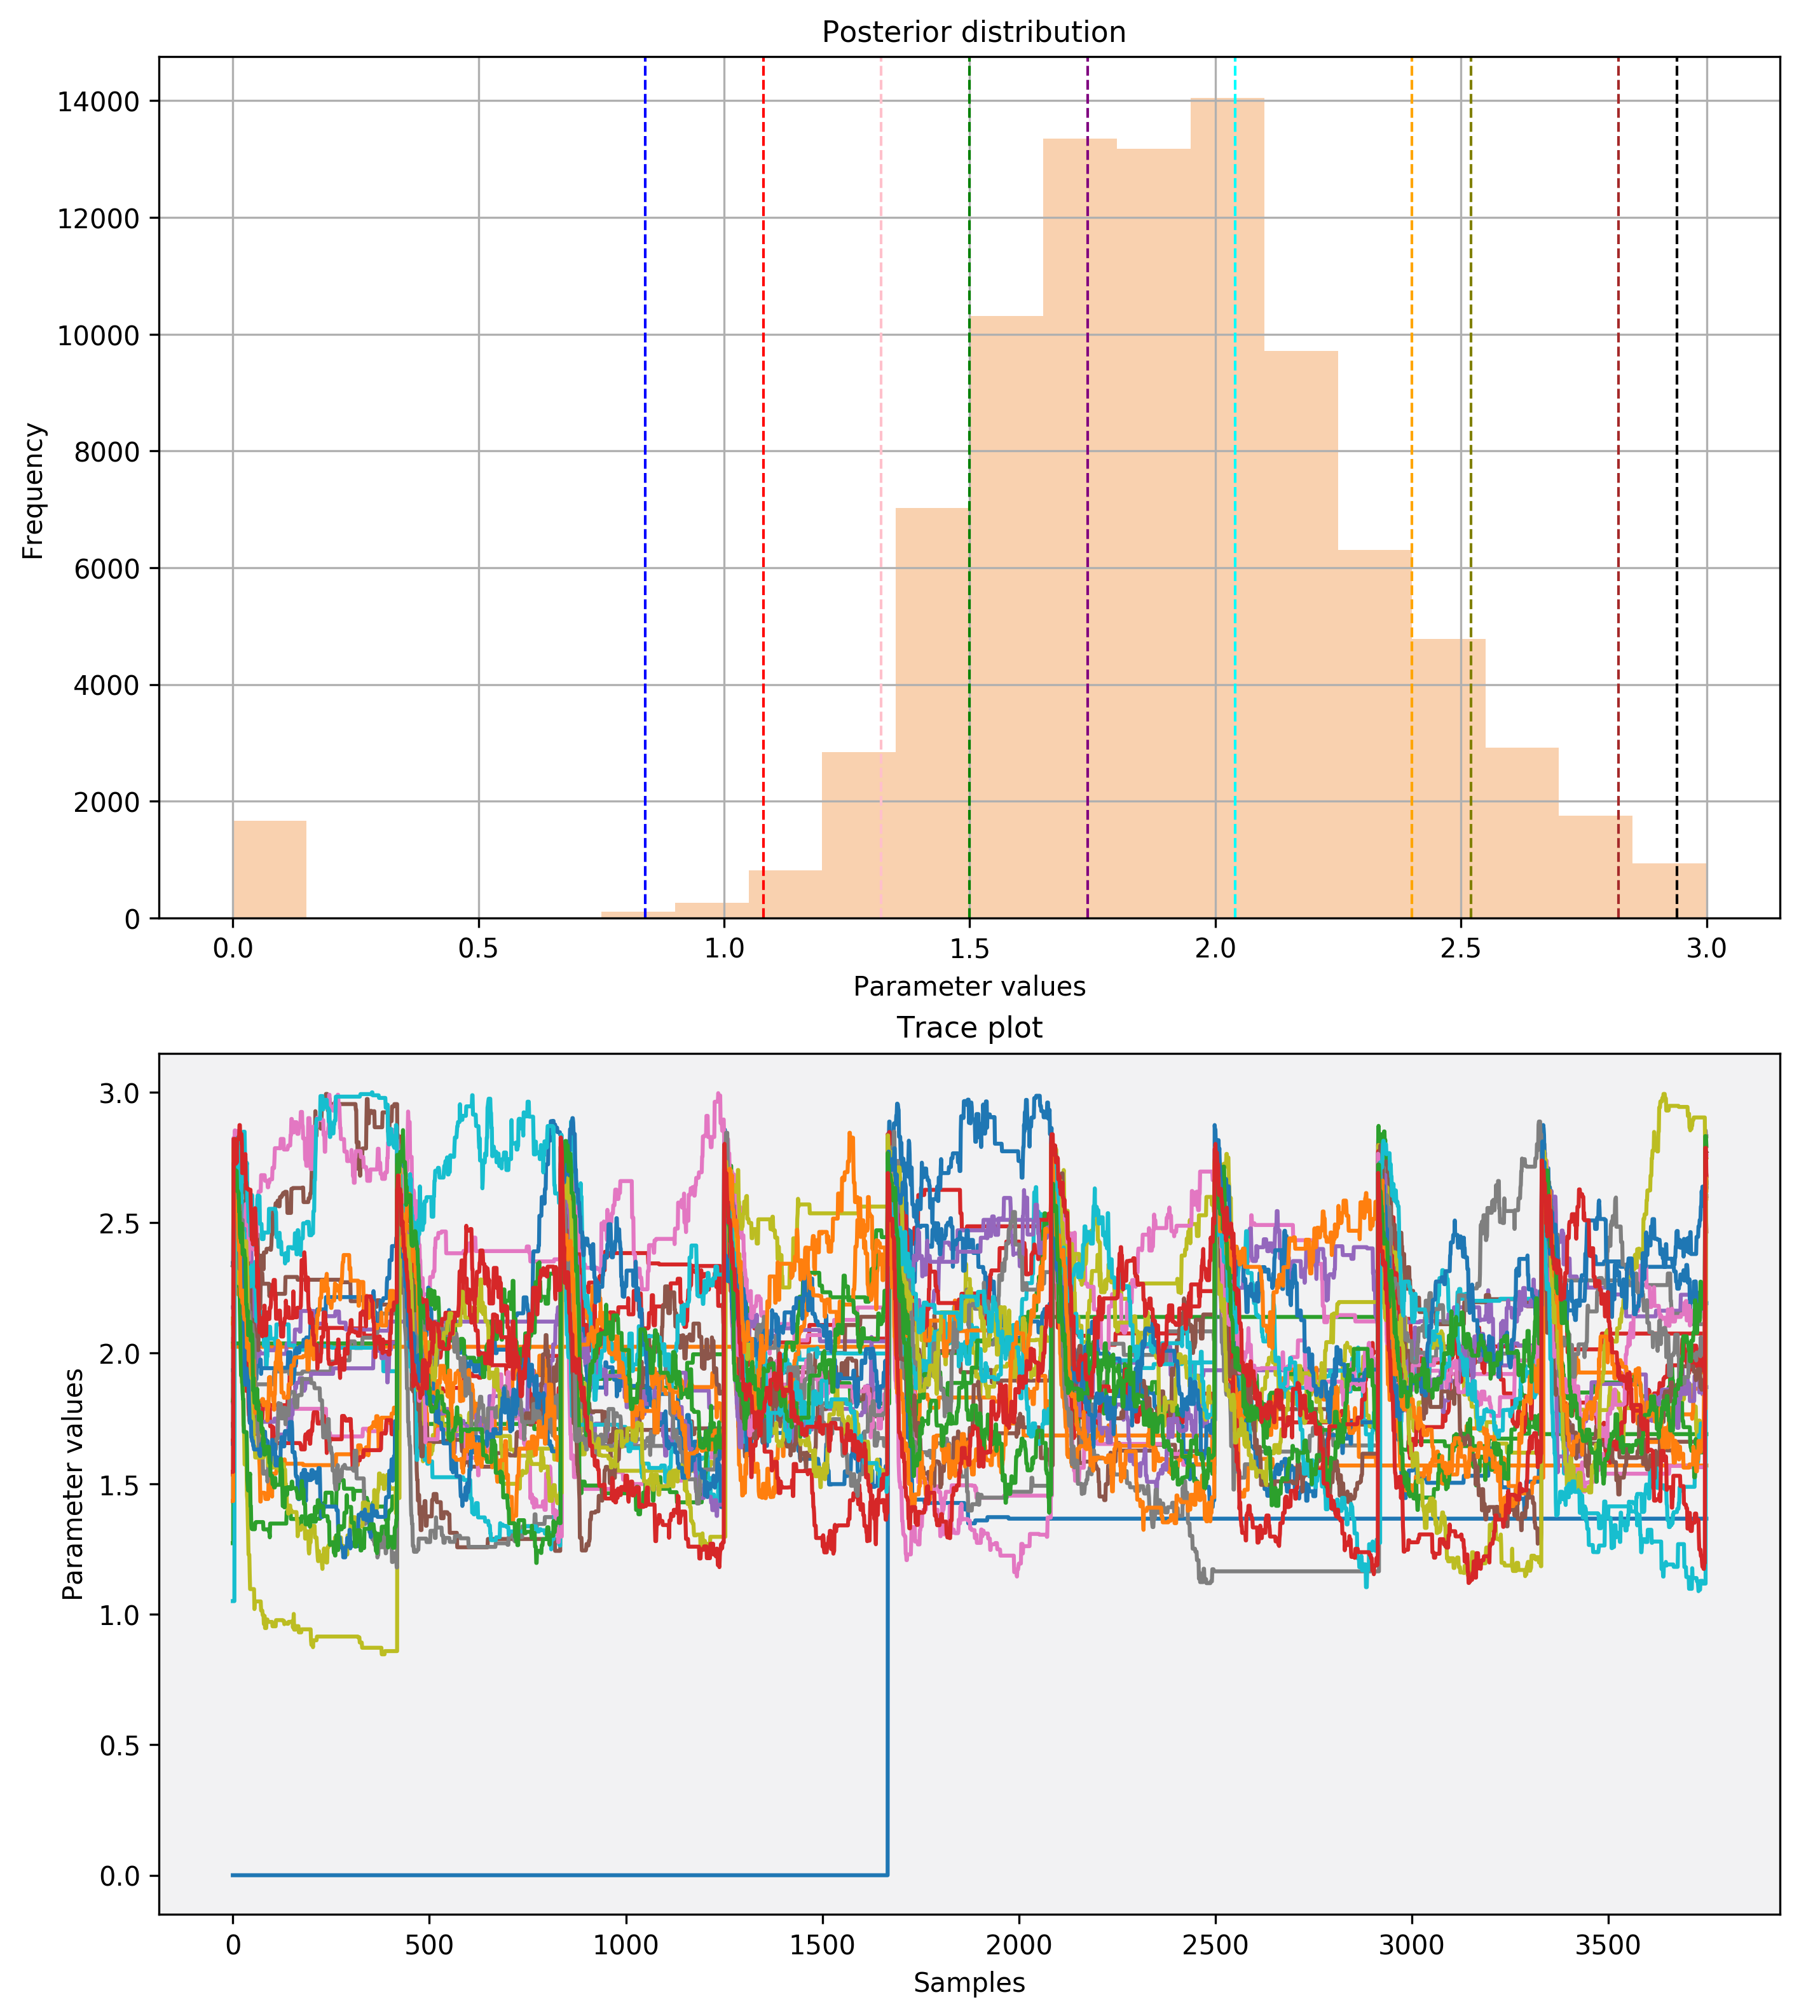
\includegraphics[width=70mm]{crater_fast/pos_distri_0_pos_.png}}
       \subfigure[Crater-short erodibility distribution]{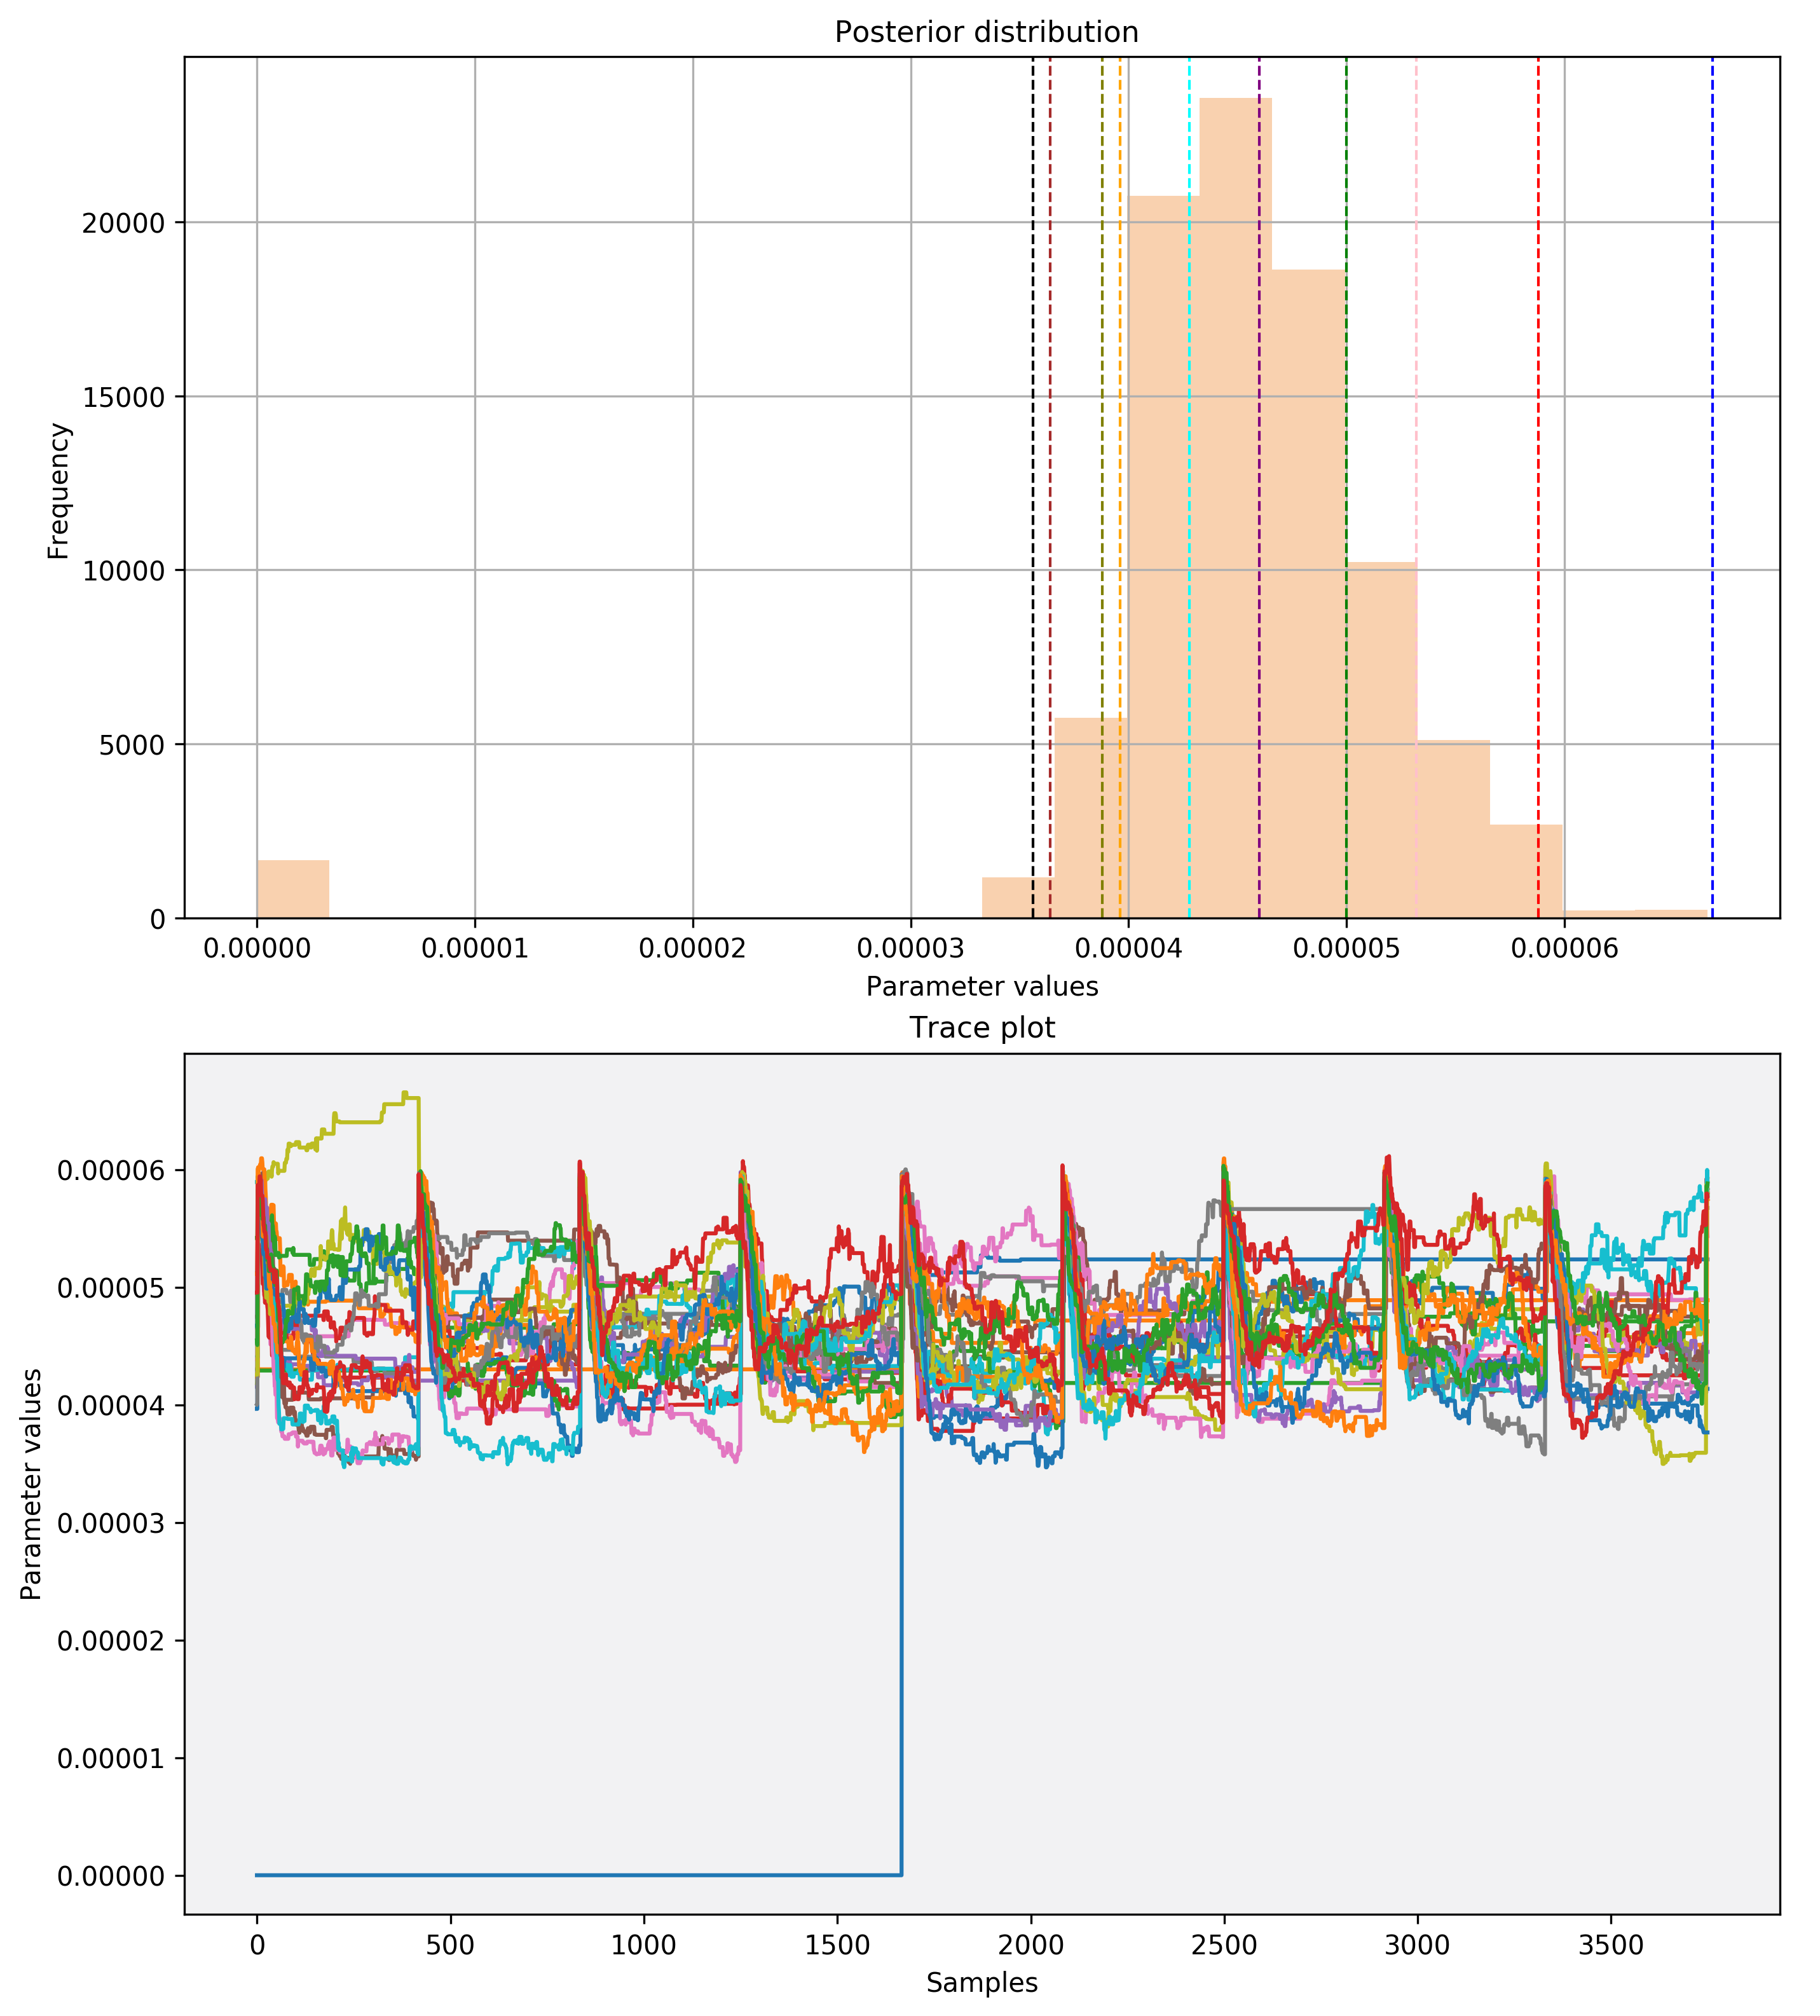
\includegraphics[width=70mm]{crater_fast/pos_distri_1_pos_.png}}\\
       \subfigure[Crater-short m distribution]{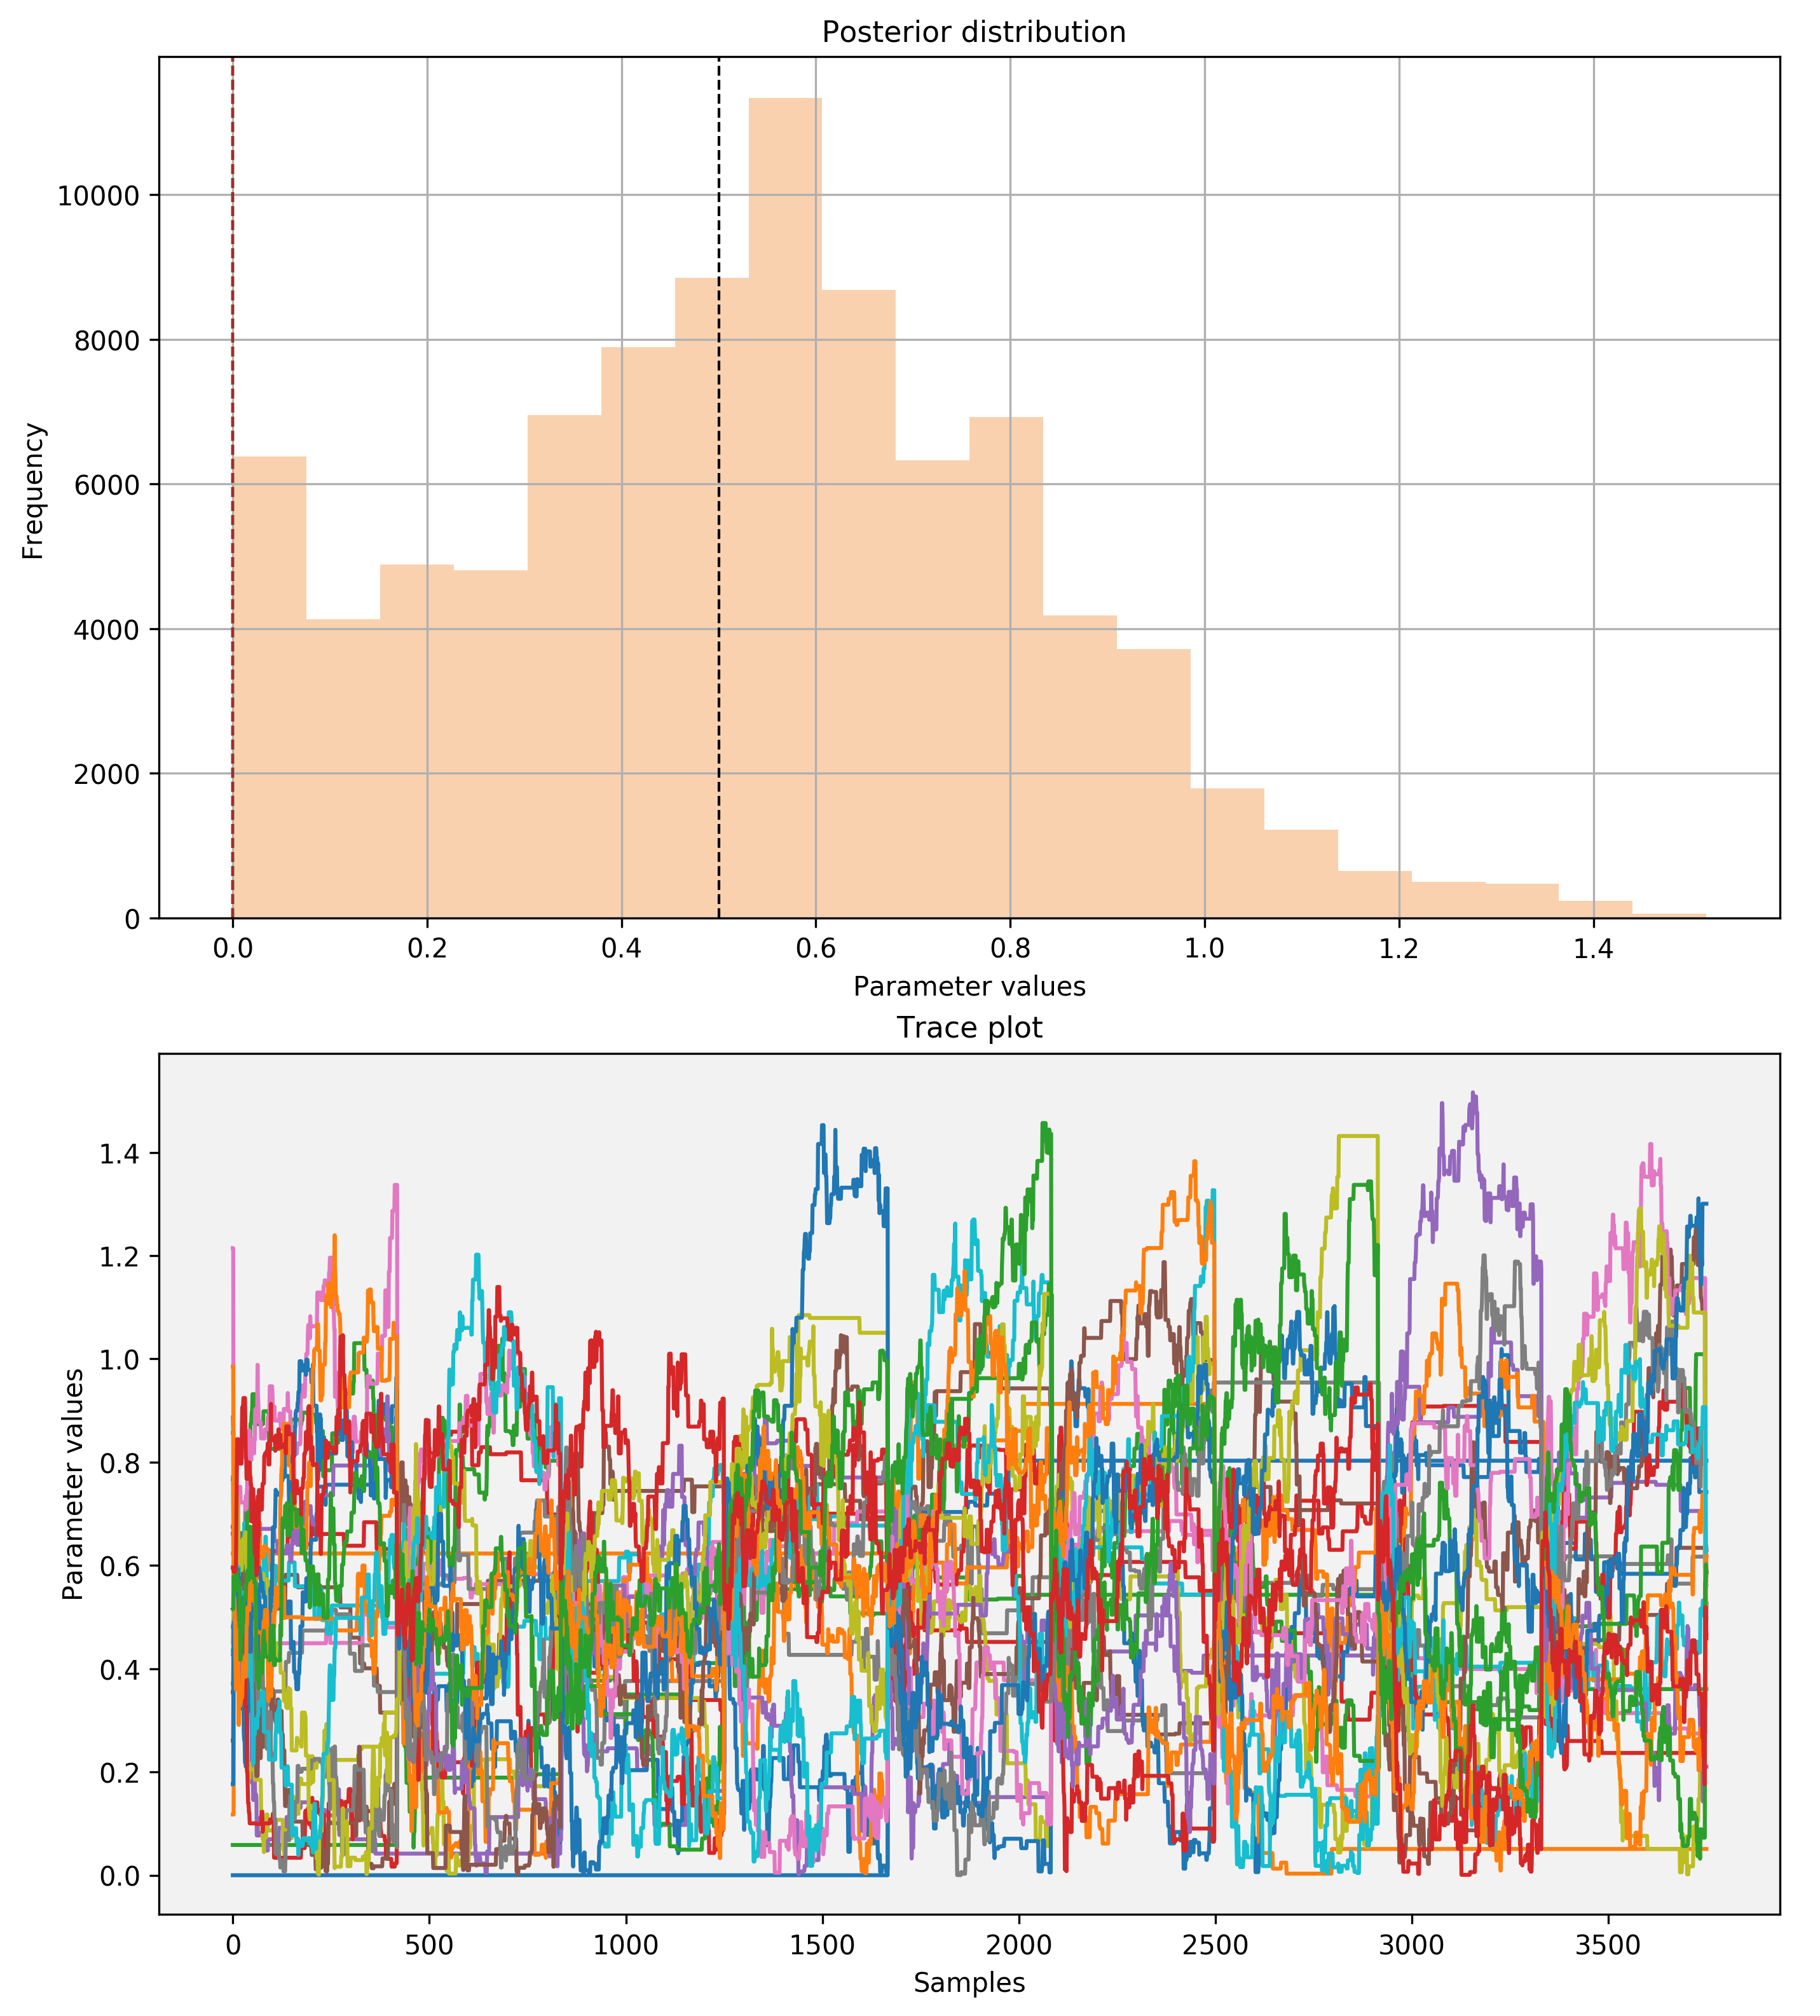
\includegraphics[width=70mm]{crater_fast/pos_distri_2_pos_.png}}
       \subfigure[Crater-short c-surface distribution]{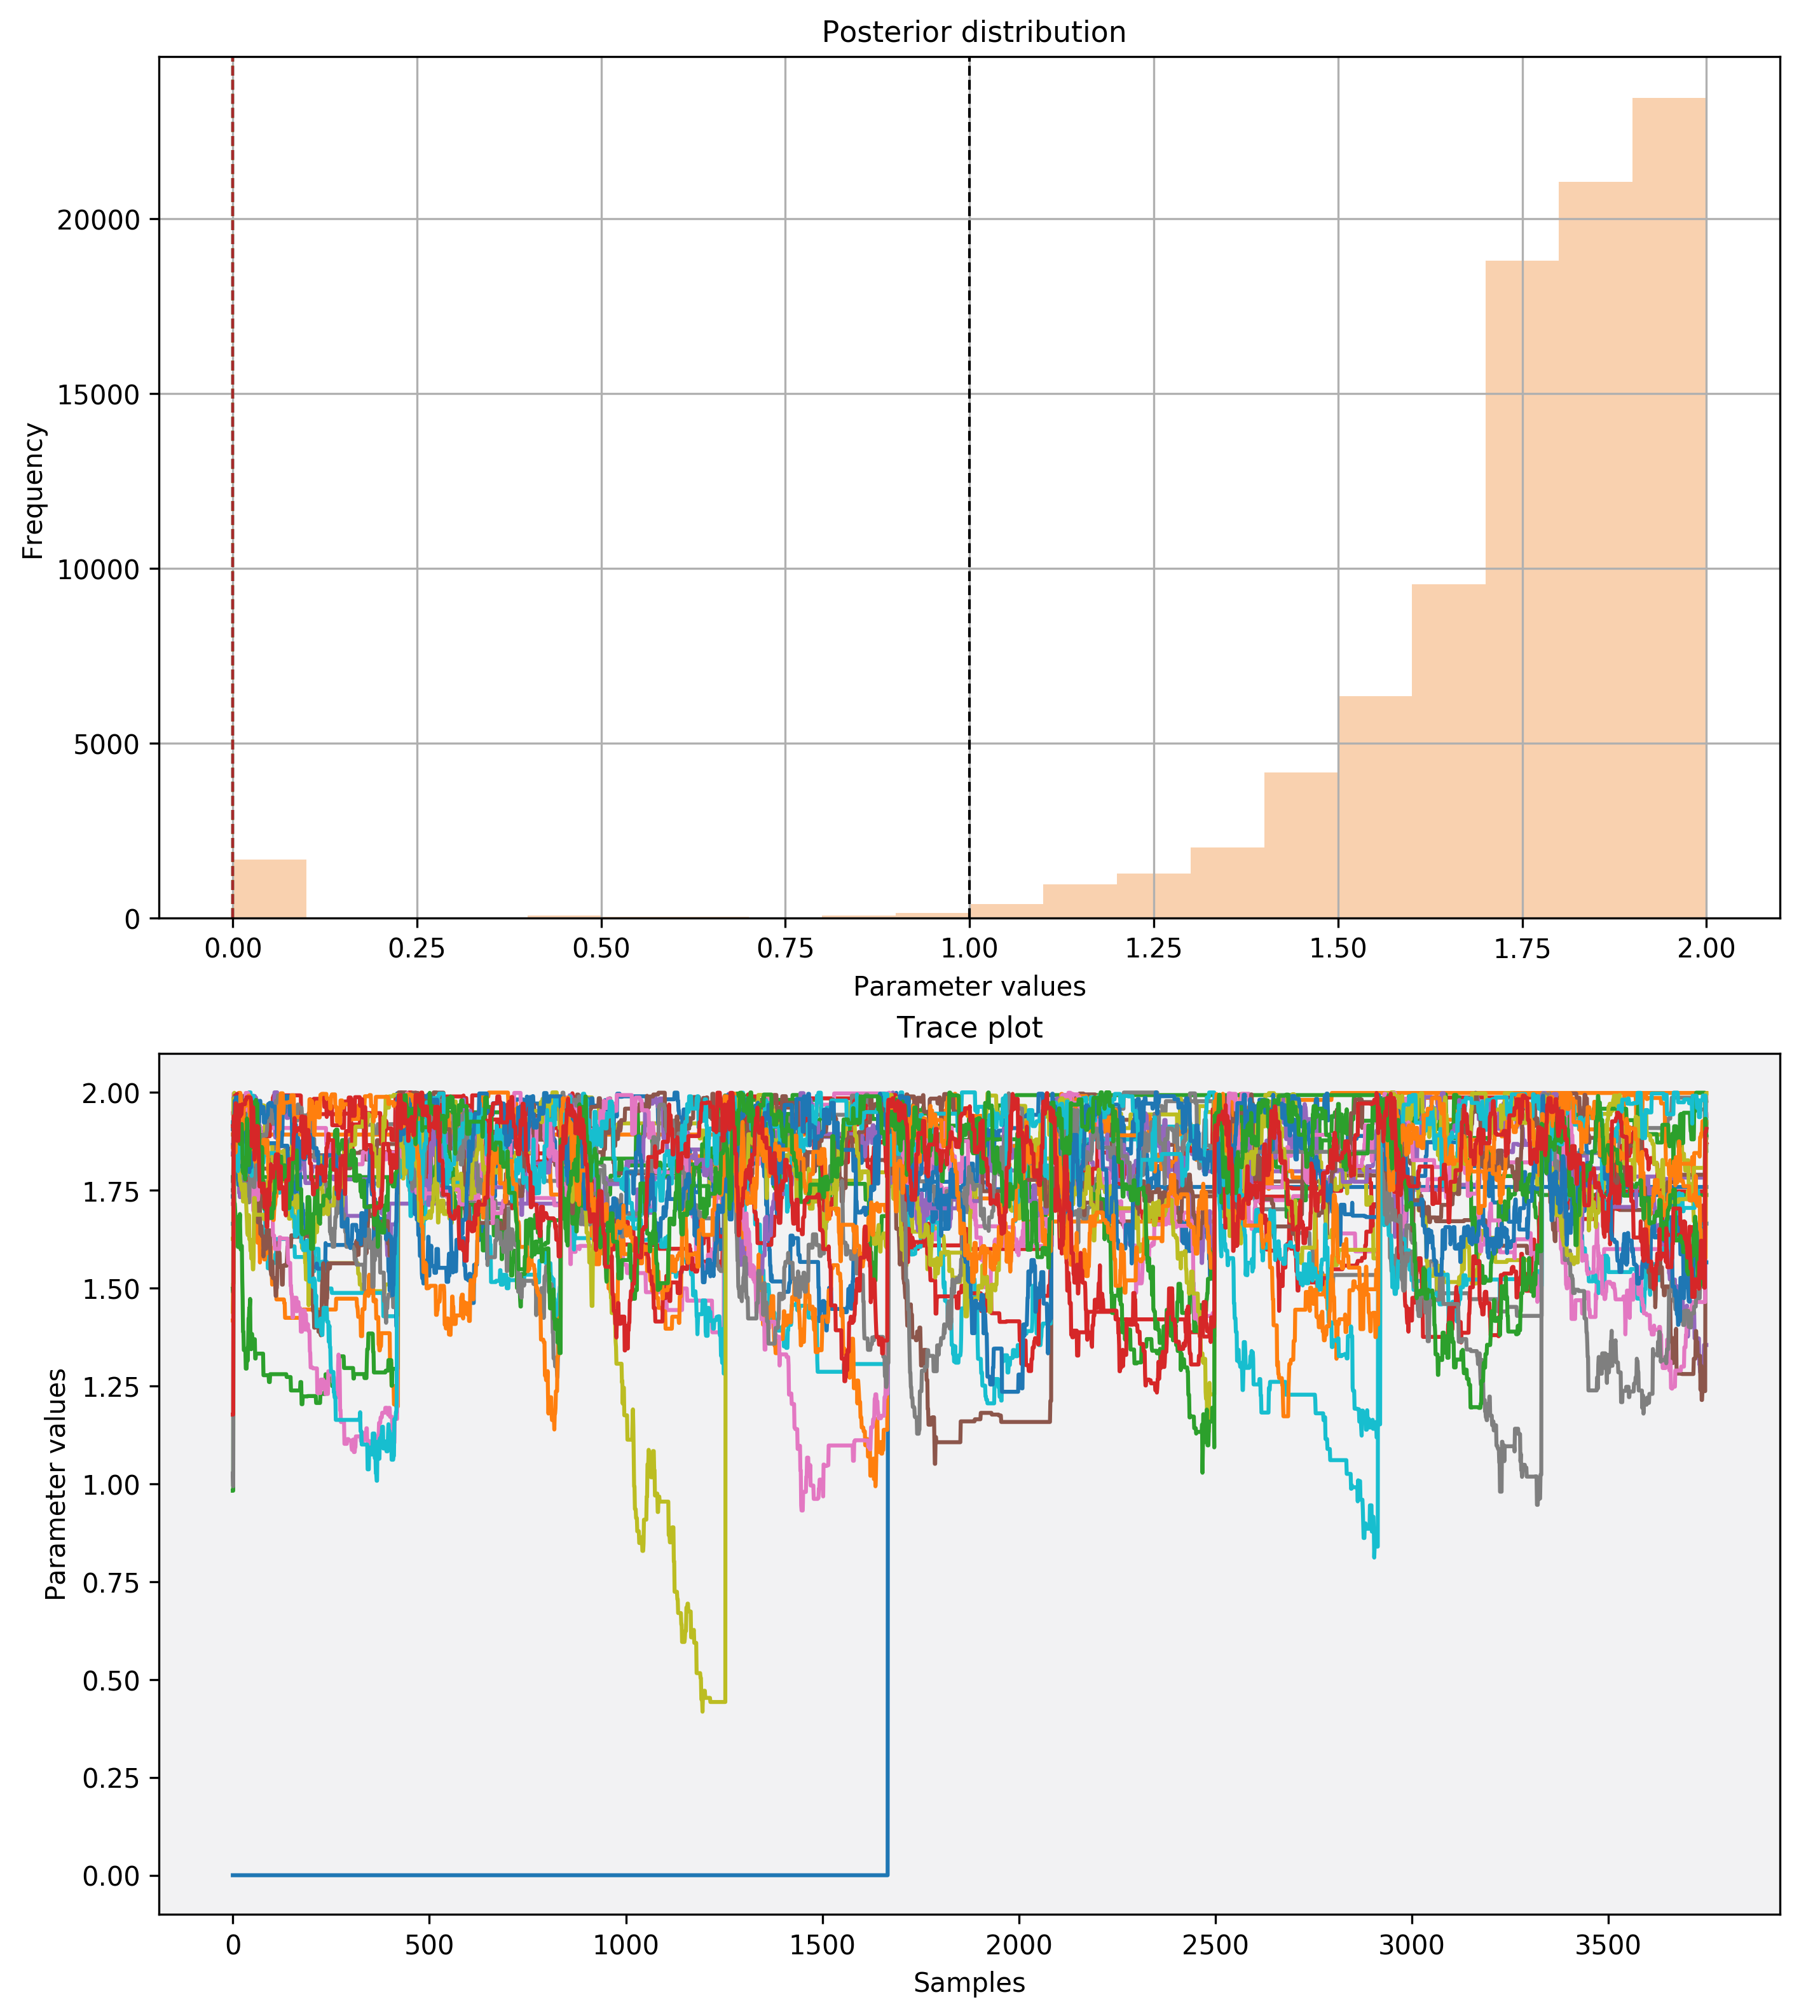
\includegraphics[width=70mm]{crater_fast/pos_distri_3_pos_.png}}\\

     \end{tabular}
     \caption{Crater-short: Posterior distribution of rainfall, erodibility, m and c-surface}
  \label{fig:crater_fast_cmarine}
}
 \end{figure*}

 %----------------------------------
 % CRATER
  %-----------------------------------

  \begin{figure*}[htb!]
{
\centering
      \begin{tabular}{cc}
        \subfigure[Elevation cross-section along x-axis]{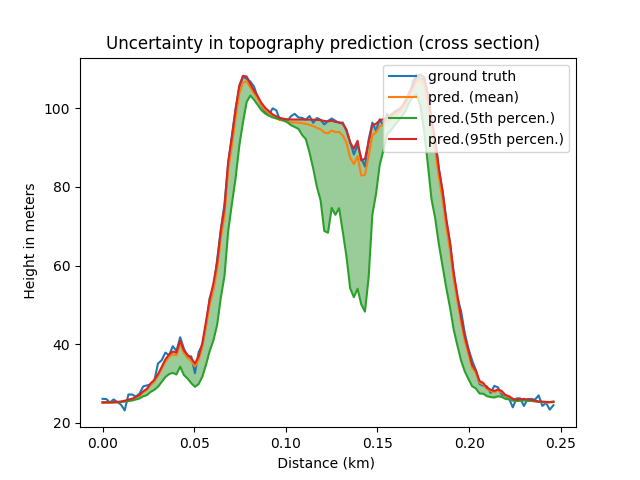
\includegraphics[width=70mm]{crater/x_ymid_opt.png}}
        \subfigure[Elevation cross-section along y-axis]{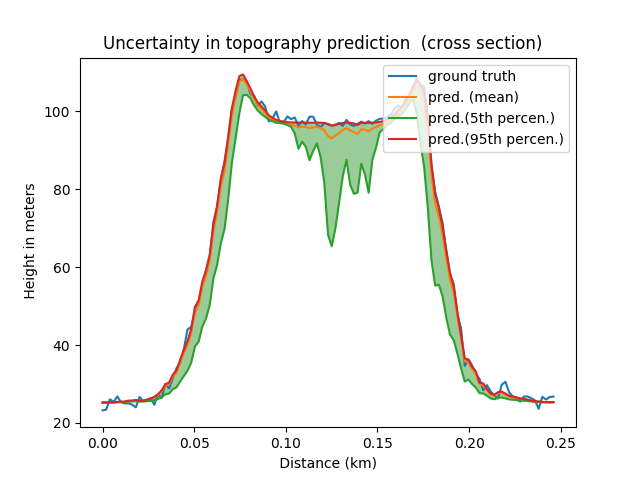
\includegraphics[width=70mm]{crater/y_xmid_opt.png}}\\
      \end{tabular}
      \caption{crater: Elevation cross-section taken at mid-point along x-axis and y-axis }
   \label{fig:crater_cross}
}
  \end{figure*}


  %-----------------------------------

 \begin{figure*}[htb!]
{
\centering
     \begin{tabular}{cc}
       \subfigure[crater erosion-deposition after 25 \% evolution time ]{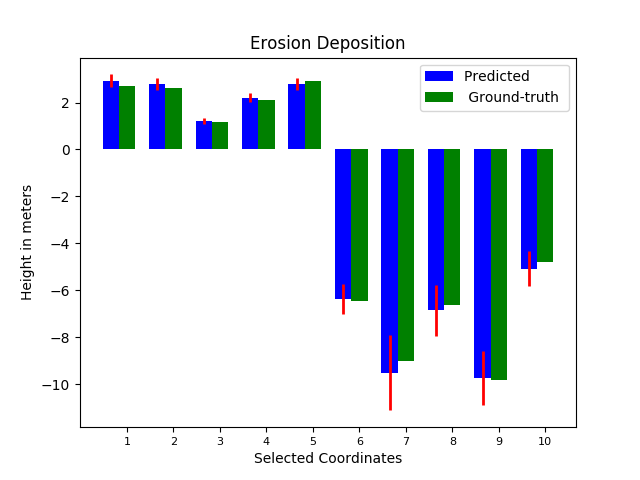
\includegraphics[width=80mm]{crater/pos_erodep_12500.png}}
       \subfigure[crater erosion-deposition  after 50 \% evolution time]{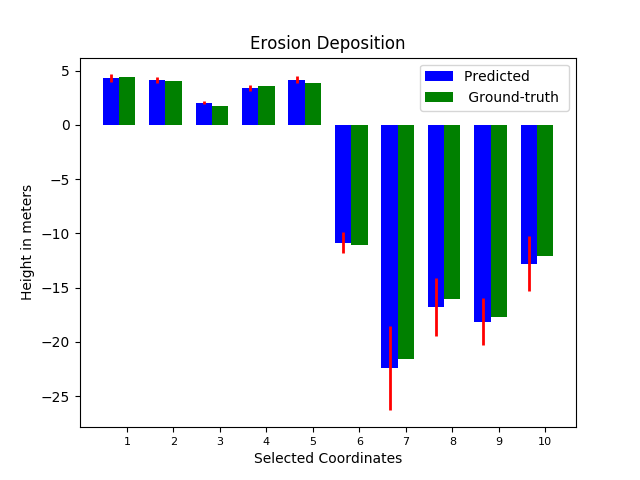
\includegraphics[width=80mm]{crater/pos_erodep_25000.png}}\\
        \subfigure[crater erosion-deposition after 75 \% evolution time ]{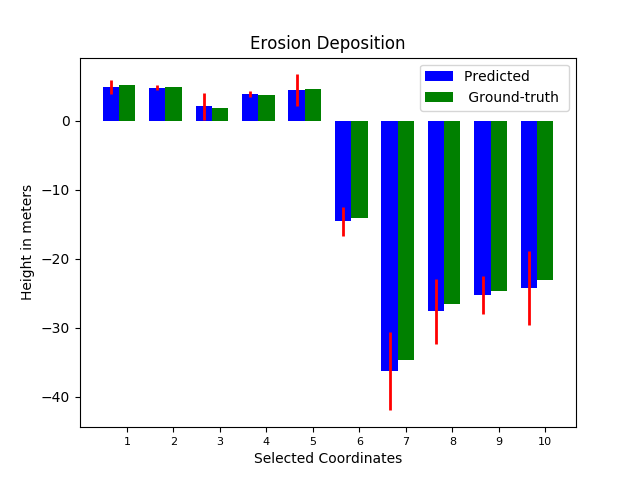
\includegraphics[width=80mm]{crater/pos_erodep_37500.png}}
       \subfigure[crater erosion-deposition  after 100 \% evolution time]{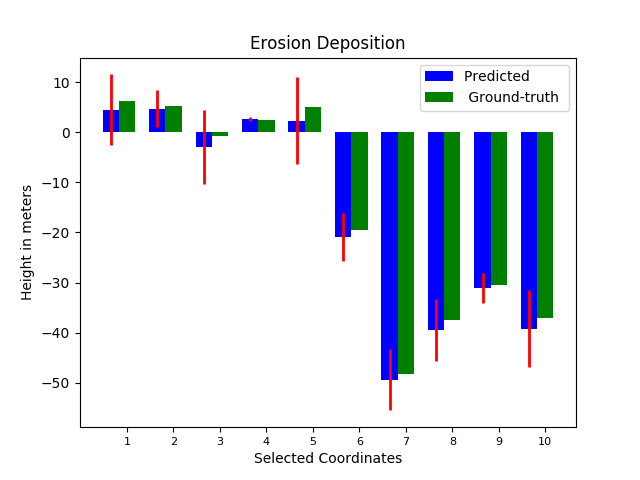
\includegraphics[width=80mm]{crater/pos_erodep_50000.png}}\\
     \end{tabular}
     \caption{crater erosion-deposition   }
  \label{fig:crater_erodep}
}
 \end{figure*}


 %----------------------------------

 \begin{figure*}[htb!]
{
\centering
     \begin{tabular}{cc}
       \subfigure[crater rainfall distribution]{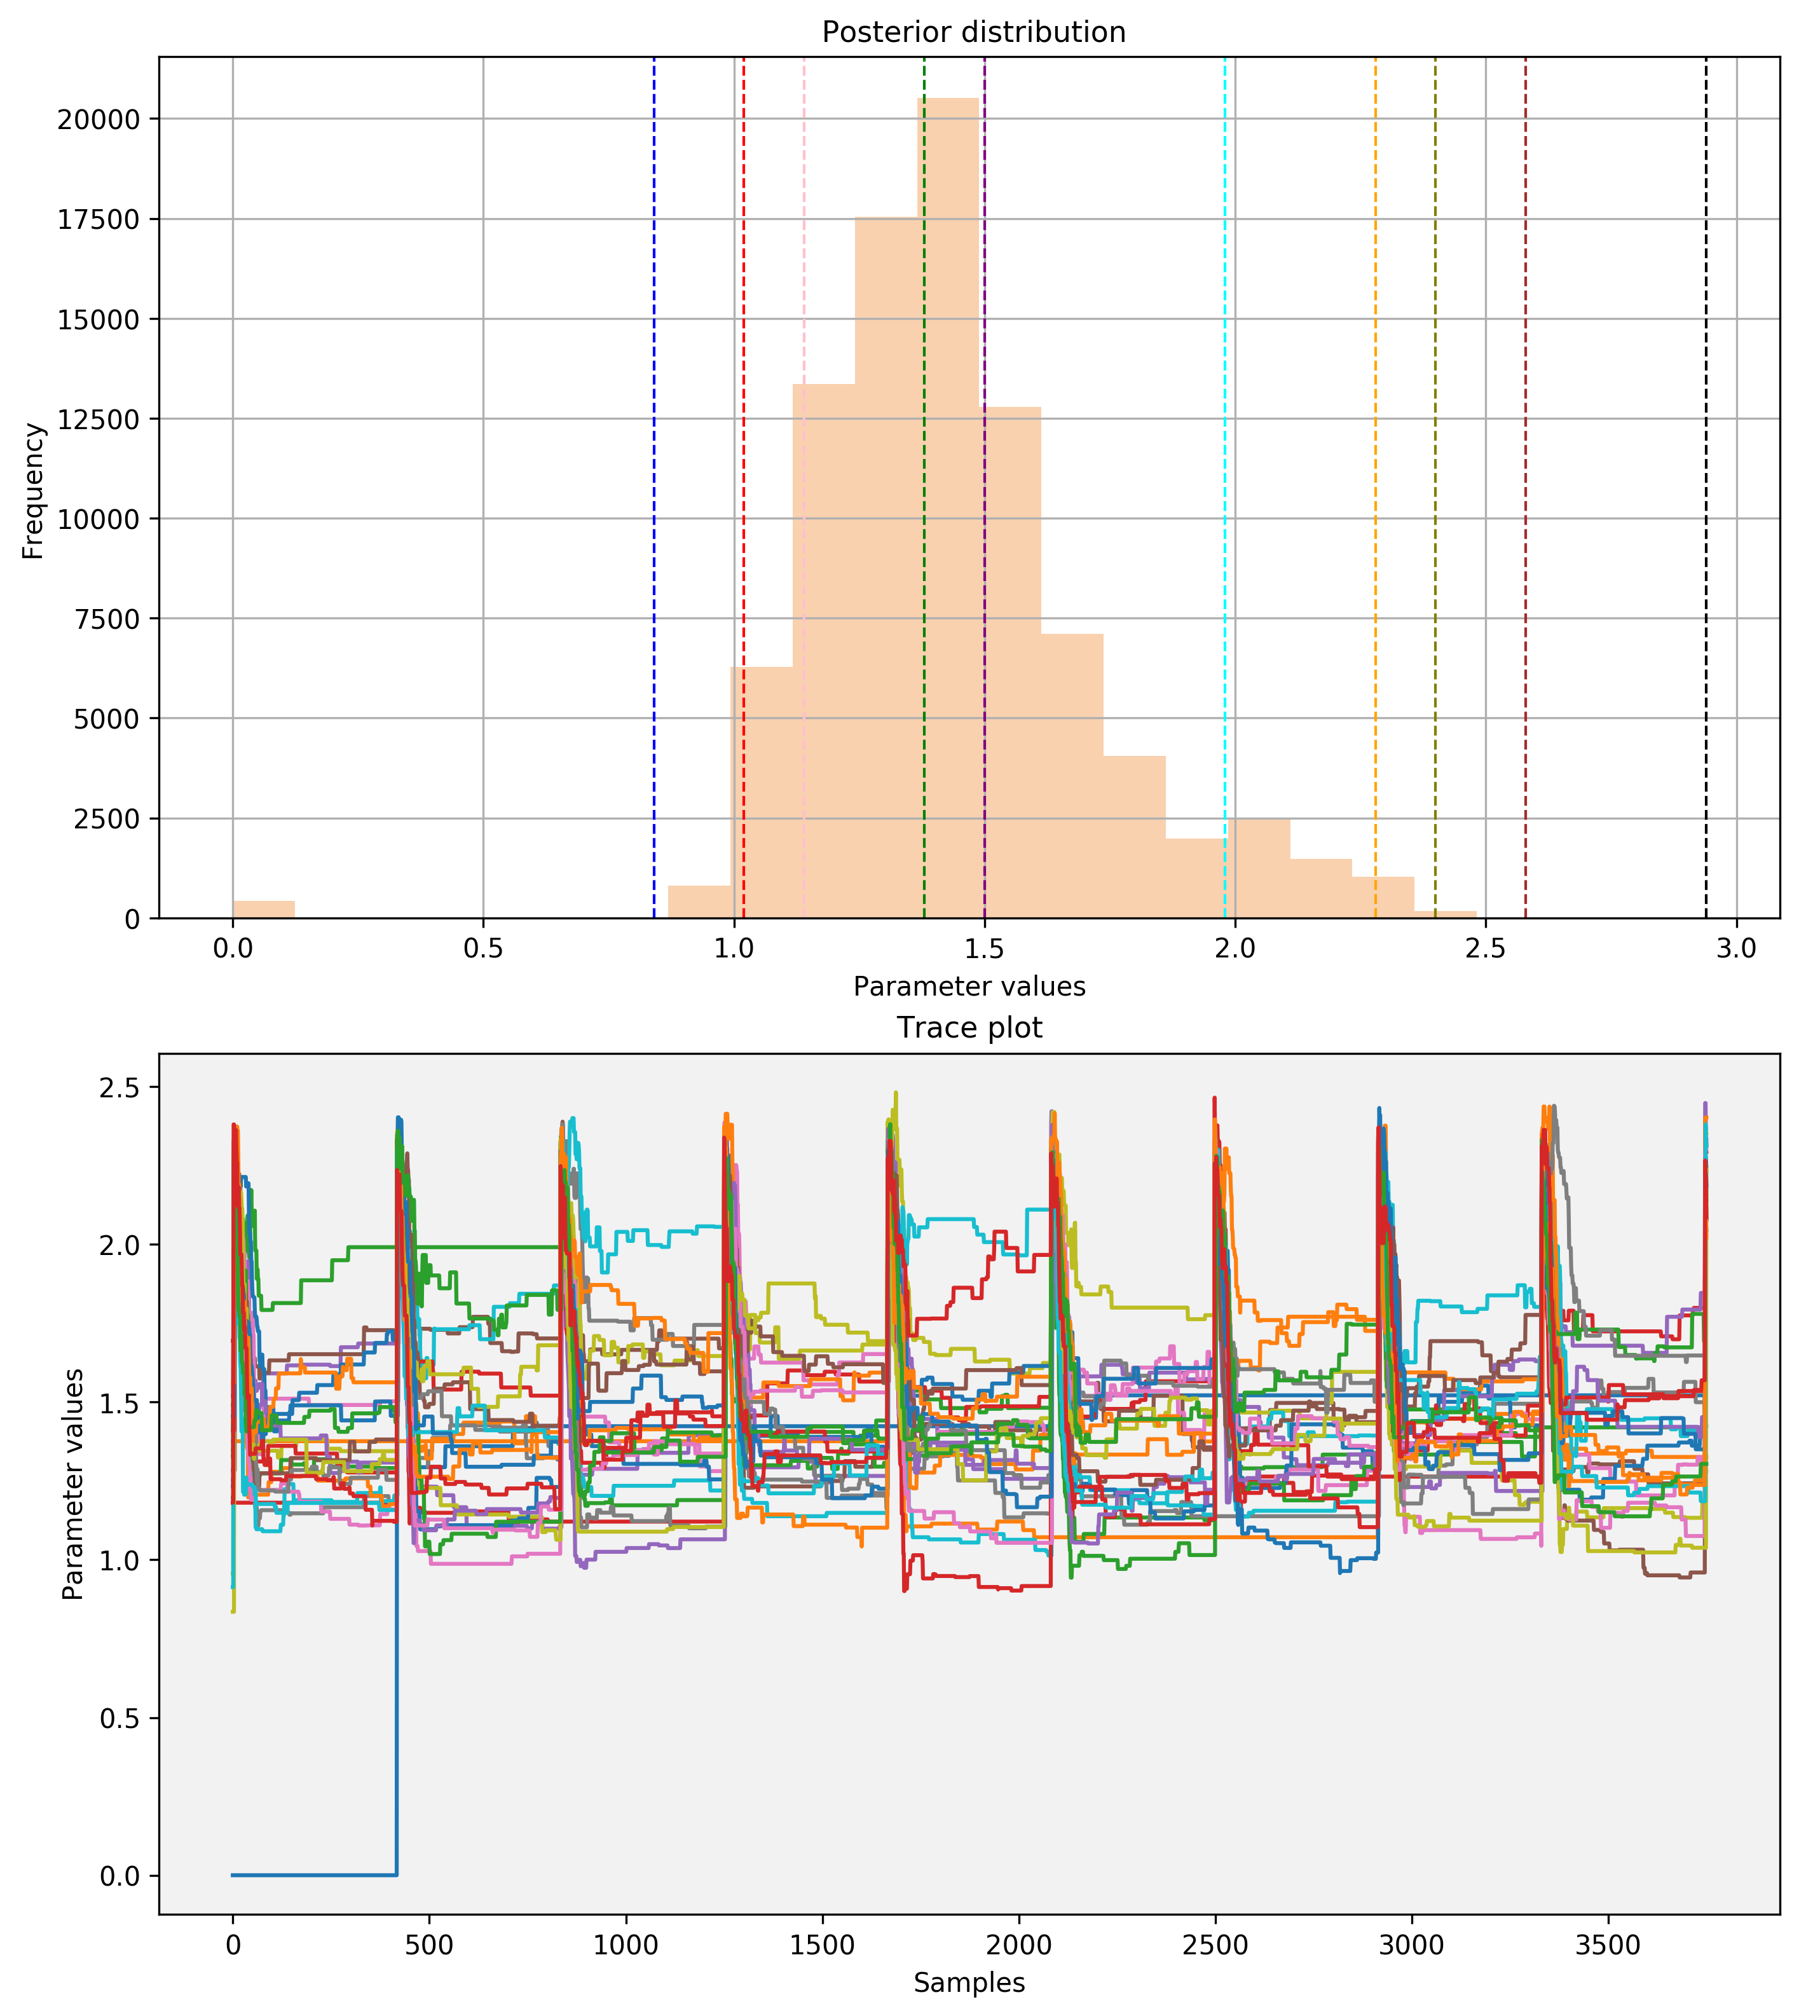
\includegraphics[width=70mm]{crater/pos_distri_0_pos_.png}}
       \subfigure[crater erodibility distribution]{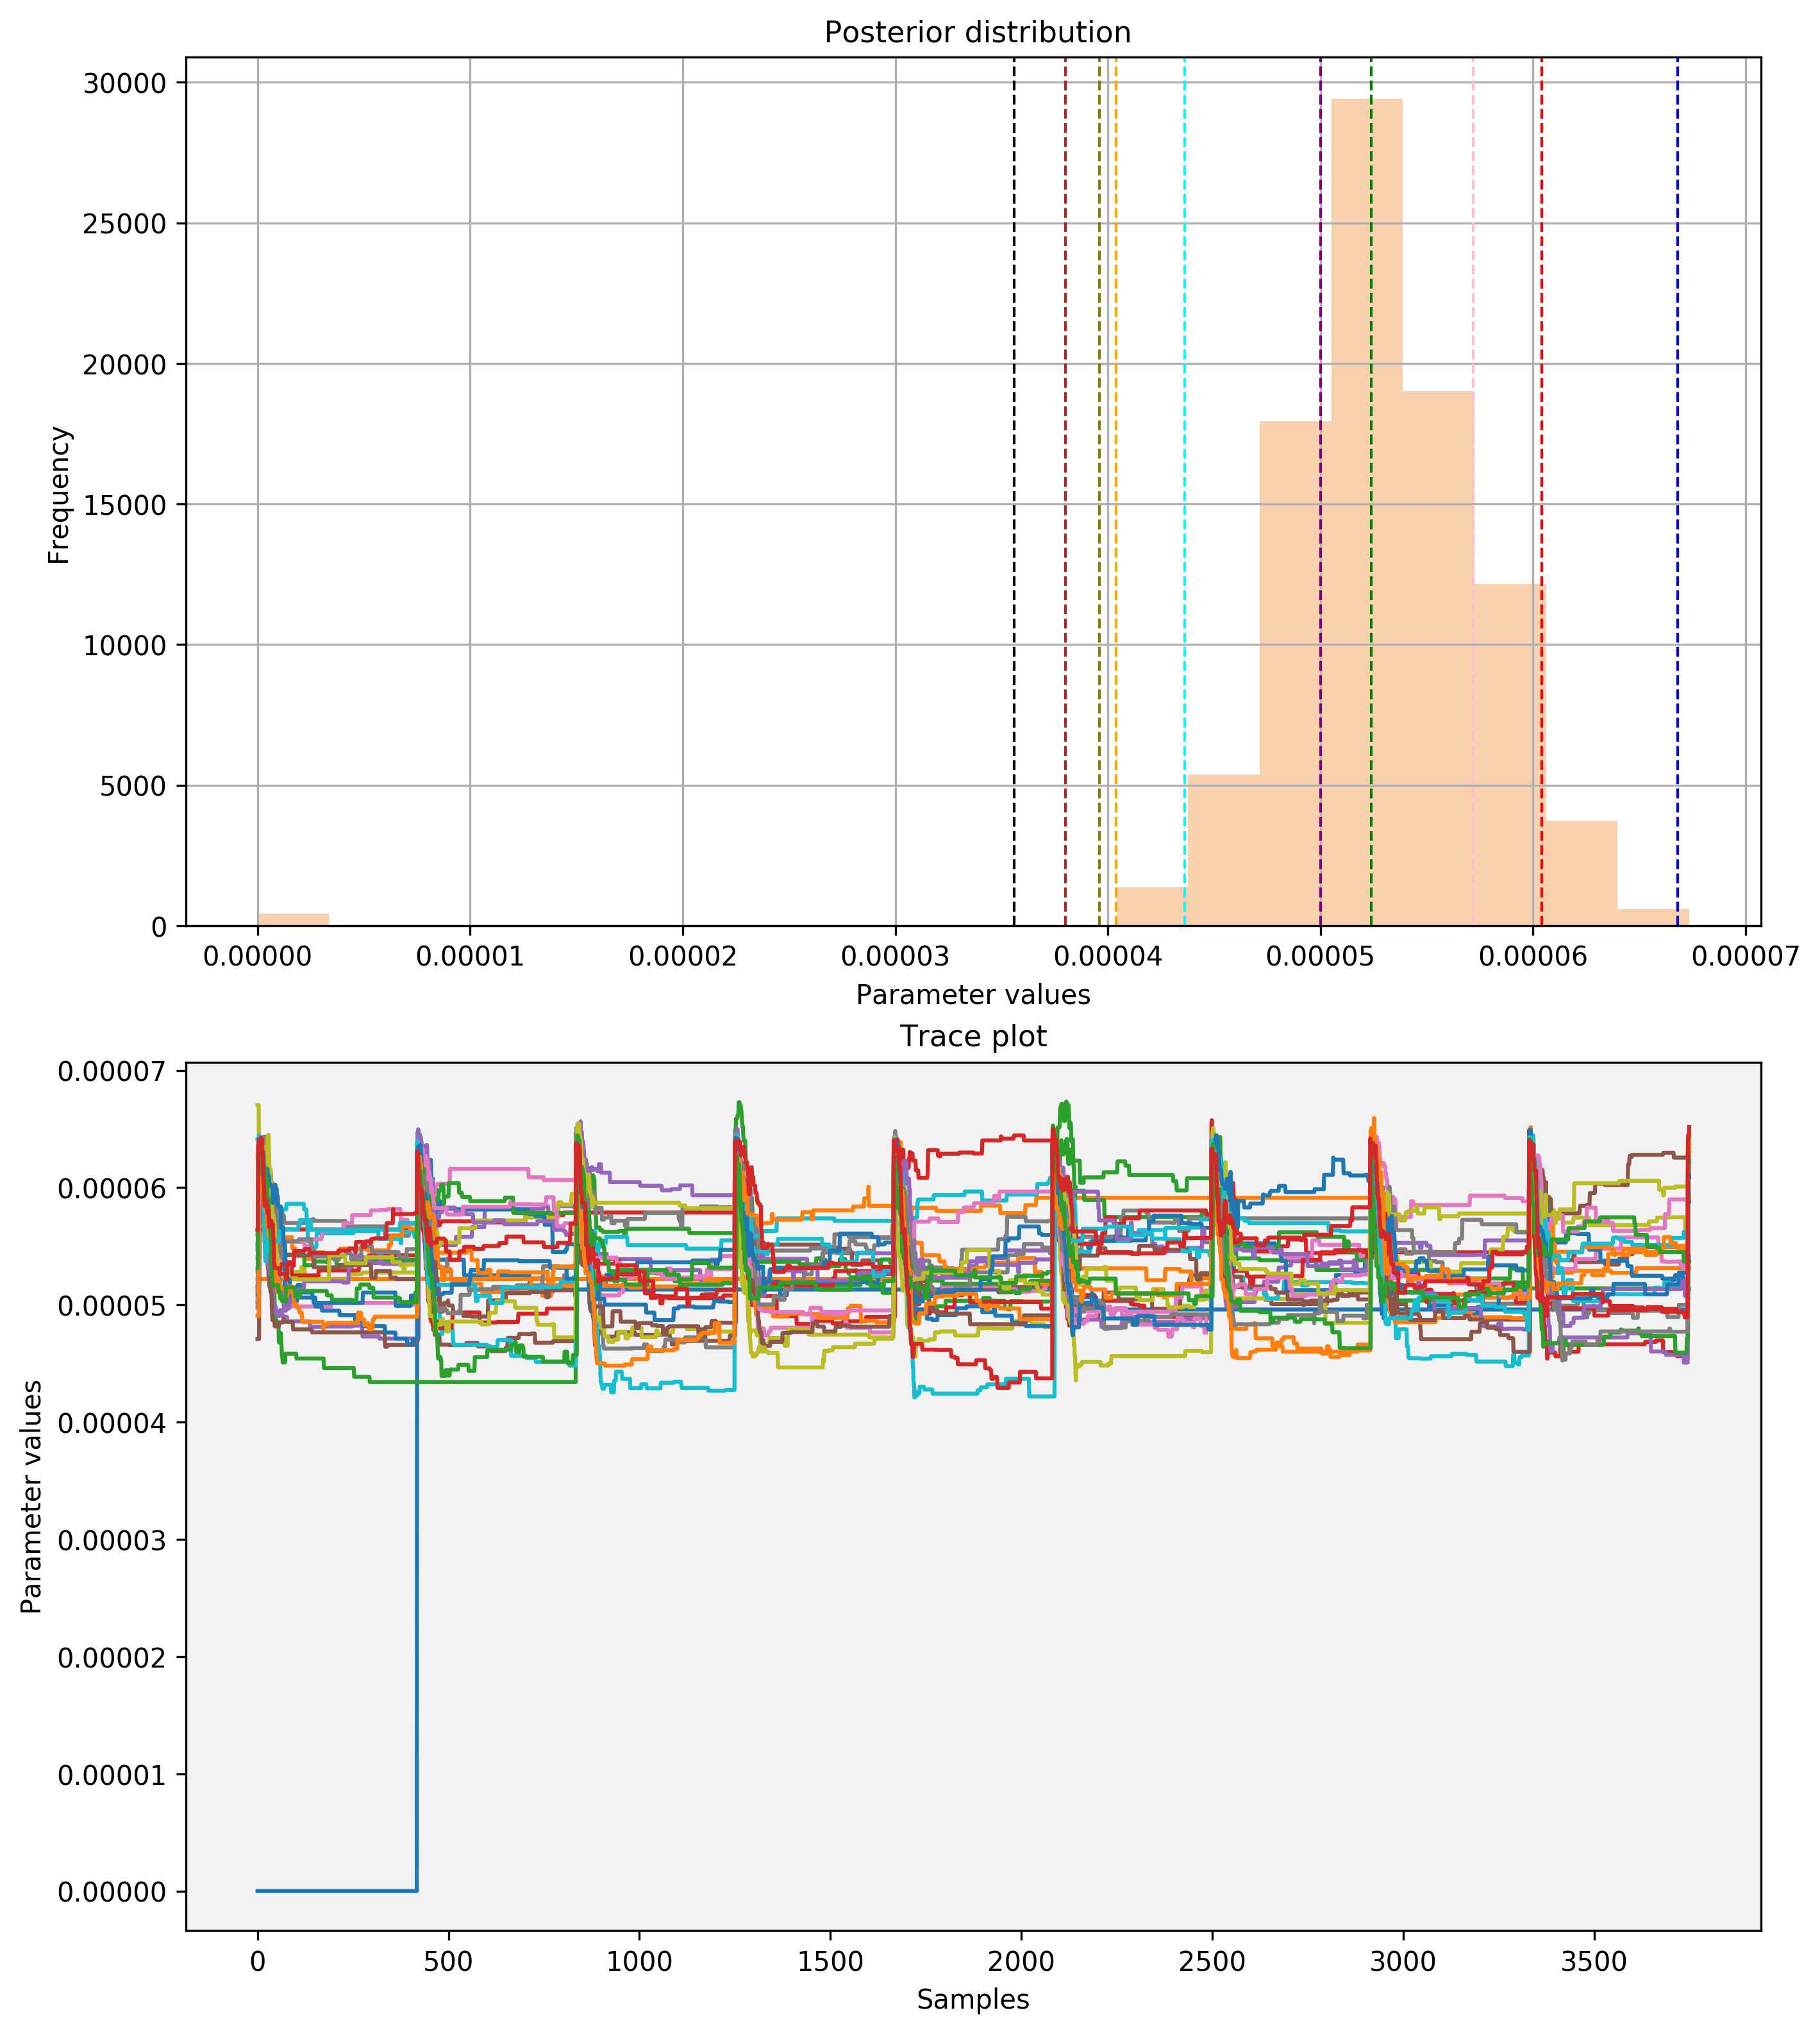
\includegraphics[width=70mm]{crater/pos_distri_1_pos_.png}}\\
       \subfigure[crater m distribution]{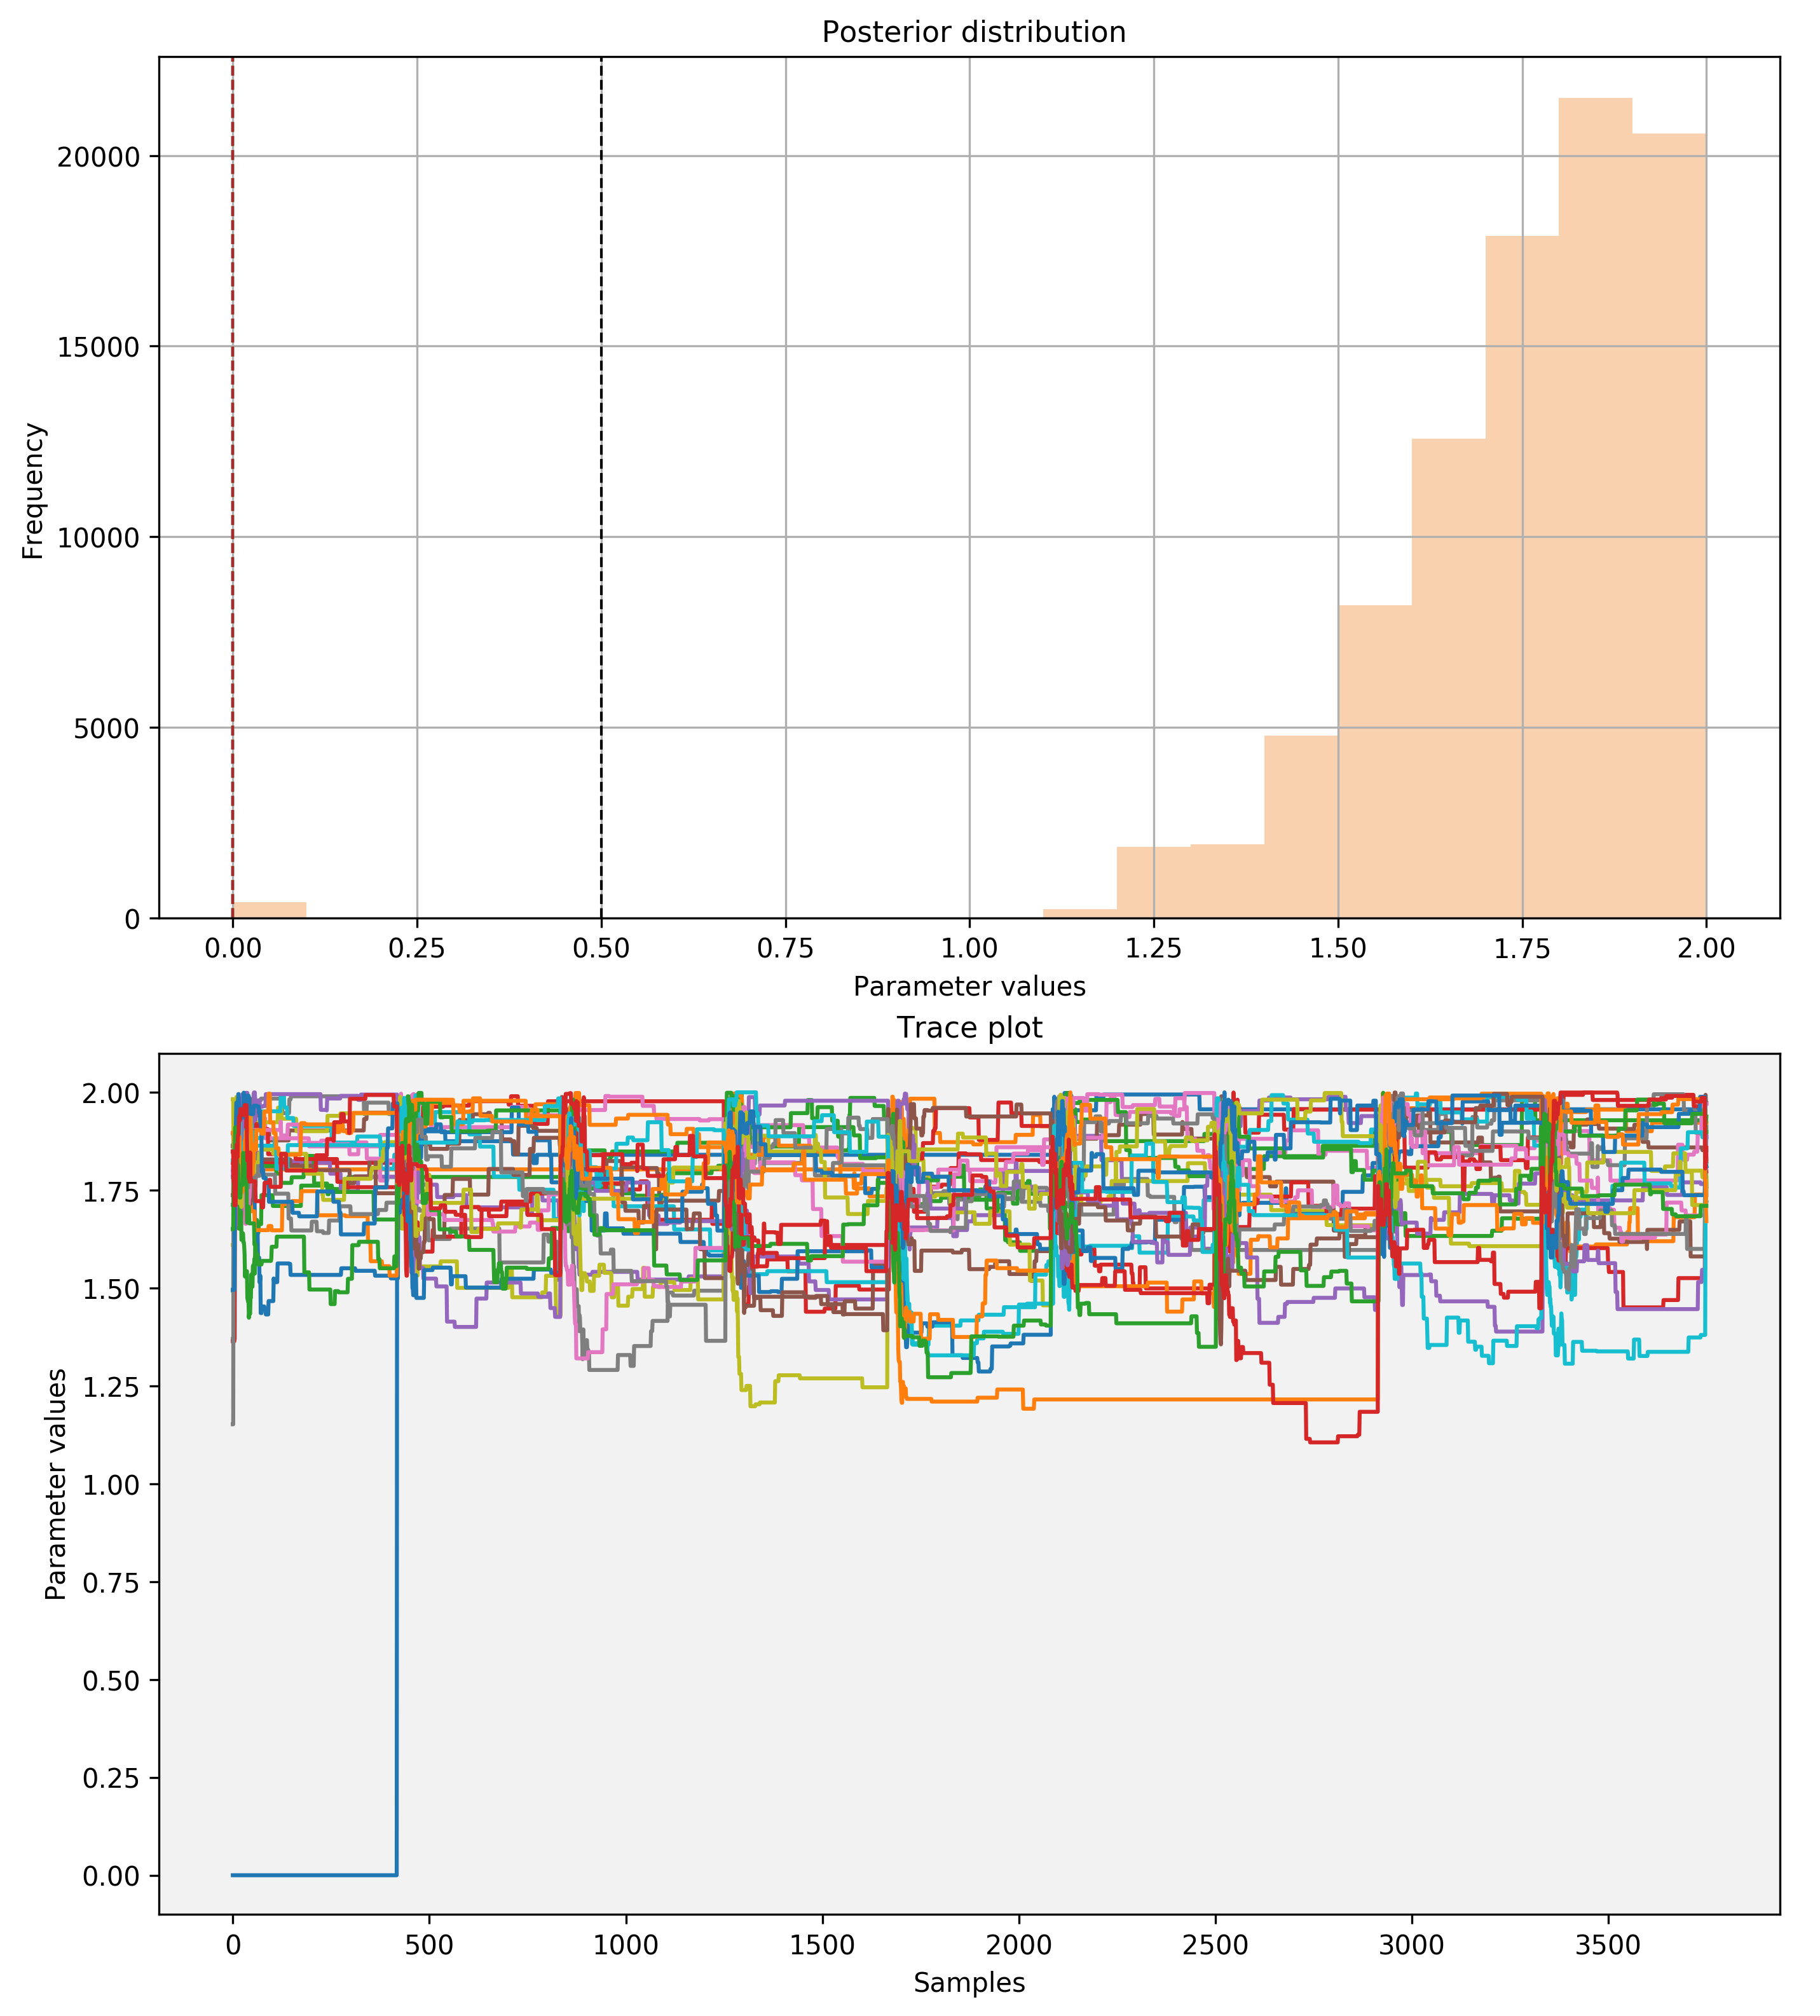
\includegraphics[width=70mm]{crater/pos_distri_2_pos_.png}}
       \subfigure[crater c-surface distribution]{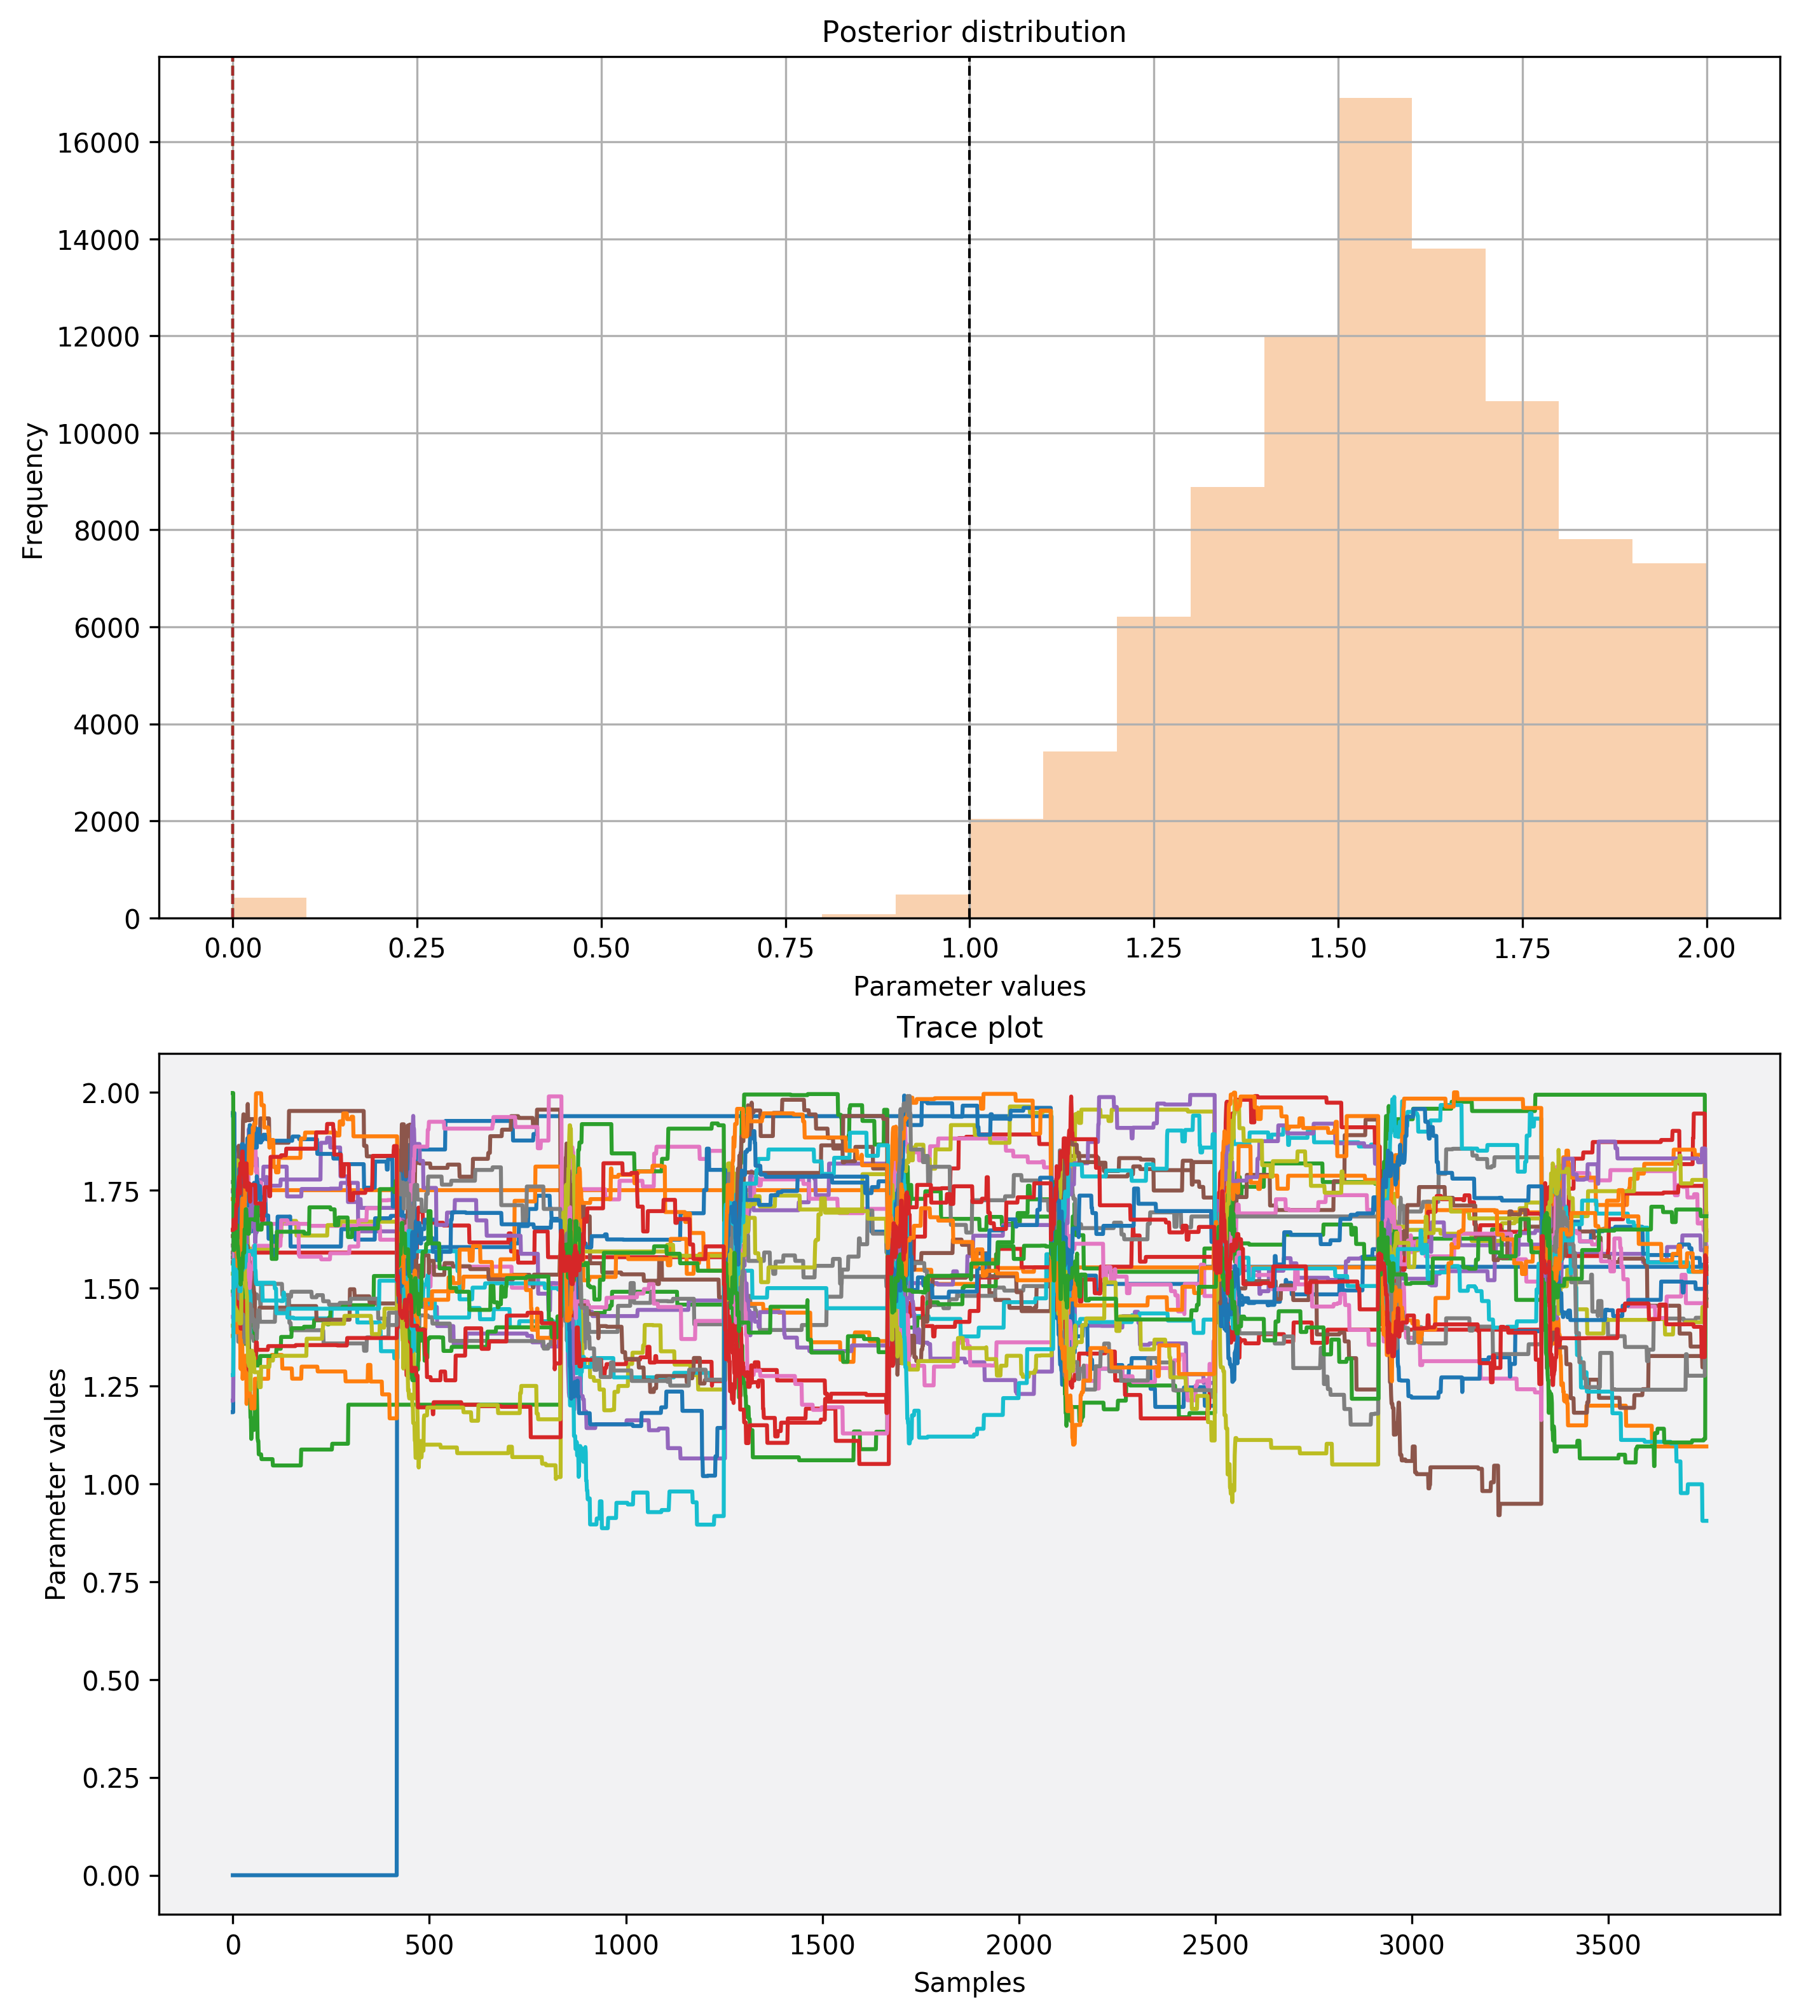
\includegraphics[width=70mm]{crater/pos_distri_3_pos_.png}}\\

     \end{tabular}
     \caption{crater: Posterior distribution of rainfall, erodibility, m and c-surface}
  \label{fig:crater_cmarine}
}
 \end{figure*}


 %------------------------------------
 % eTopo SHORT
  %-----------------------------------

  \begin{figure*}[htb!]
{
\centering
      \begin{tabular}{cc}
        \subfigure[Elevation cross-section along x-axis]{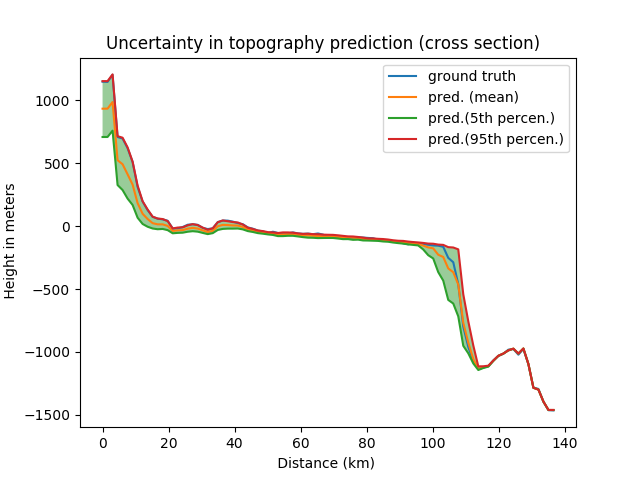
\includegraphics[width=70mm]{etopo_fast/x_ymid_opt.png}}
        \subfigure[Elevation cross-section along y-axis]{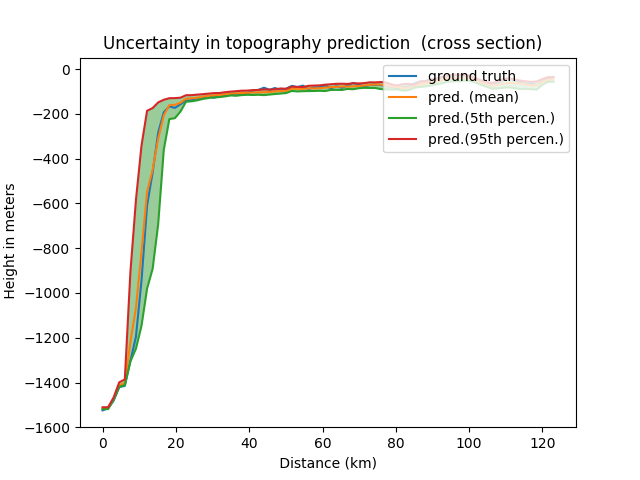
\includegraphics[width=70mm]{etopo_fast/y_xmid_opt.png}}\\
      \end{tabular}
      \caption{eTopo\_short: Elevation cross-section taken at mid-point along x-axis and y-axis }
   \label{fig:etopo_fast_cross}
}
  \end{figure*}


  %-----------------------------------

 \begin{figure*}[htb!]
{
\centering
     \begin{tabular}{cc}
       \subfigure[Etopo-short erosion-deposition after 25 \% evolution time ]{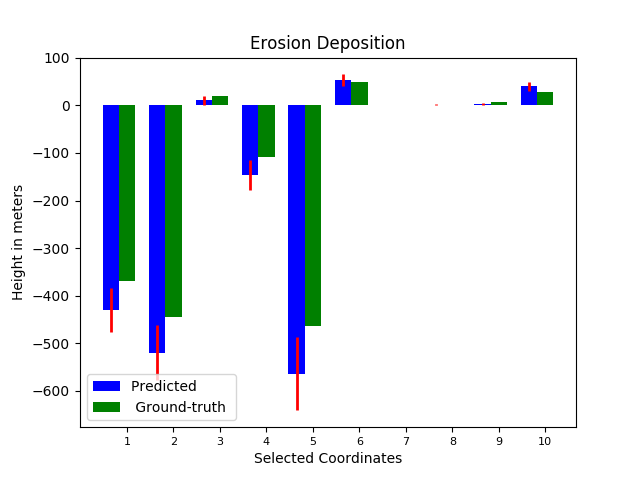
\includegraphics[width=80mm]{etopo_fast/pos_erodep_125000.png}}
       \subfigure[Etopo-short erosion-deposition  after 50 \% evolution time]{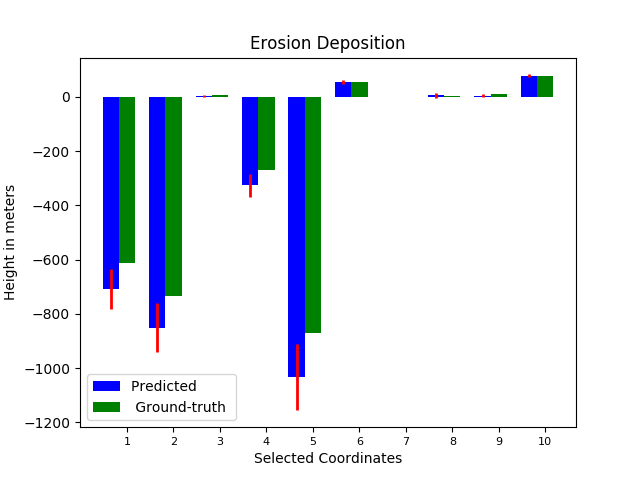
\includegraphics[width=80mm]{etopo_fast/pos_erodep_250000.png}}\\
        \subfigure[Etopo-short erosion-deposition after 75 \% evolution time ]{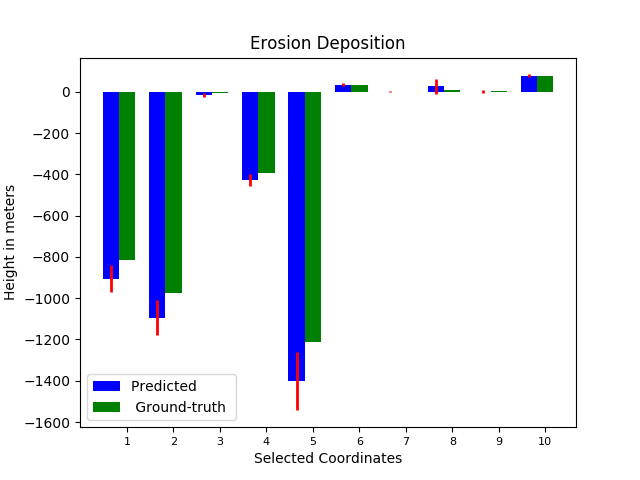
\includegraphics[width=80mm]{etopo_fast/pos_erodep_375000.png}}
       \subfigure[Etopo-short erosion-deposition  after 100 \% evolution time]{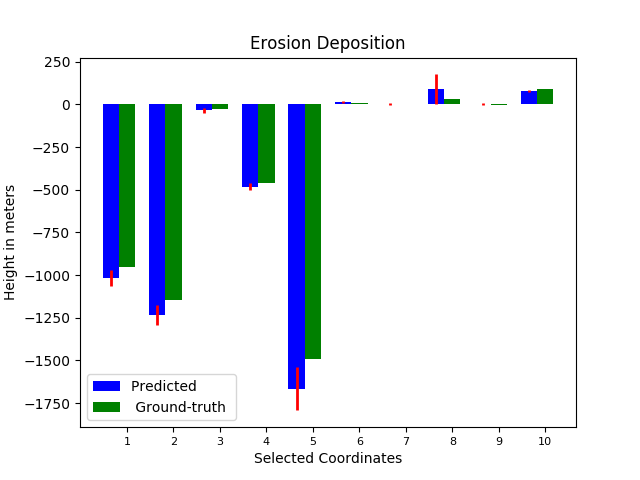
\includegraphics[width=80mm]{etopo_fast/pos_erodep_500000.png}}\\
     \end{tabular}
     \caption{Etopo-short erosion-deposition   }
  \label{fig:etopo_fast_erodep}
}
 \end{figure*}


 %----------------------------------

 \begin{figure*}[htb!]
{
\centering
     \begin{tabular}{cc}
       \subfigure[Etopo-short rainfall distribution]{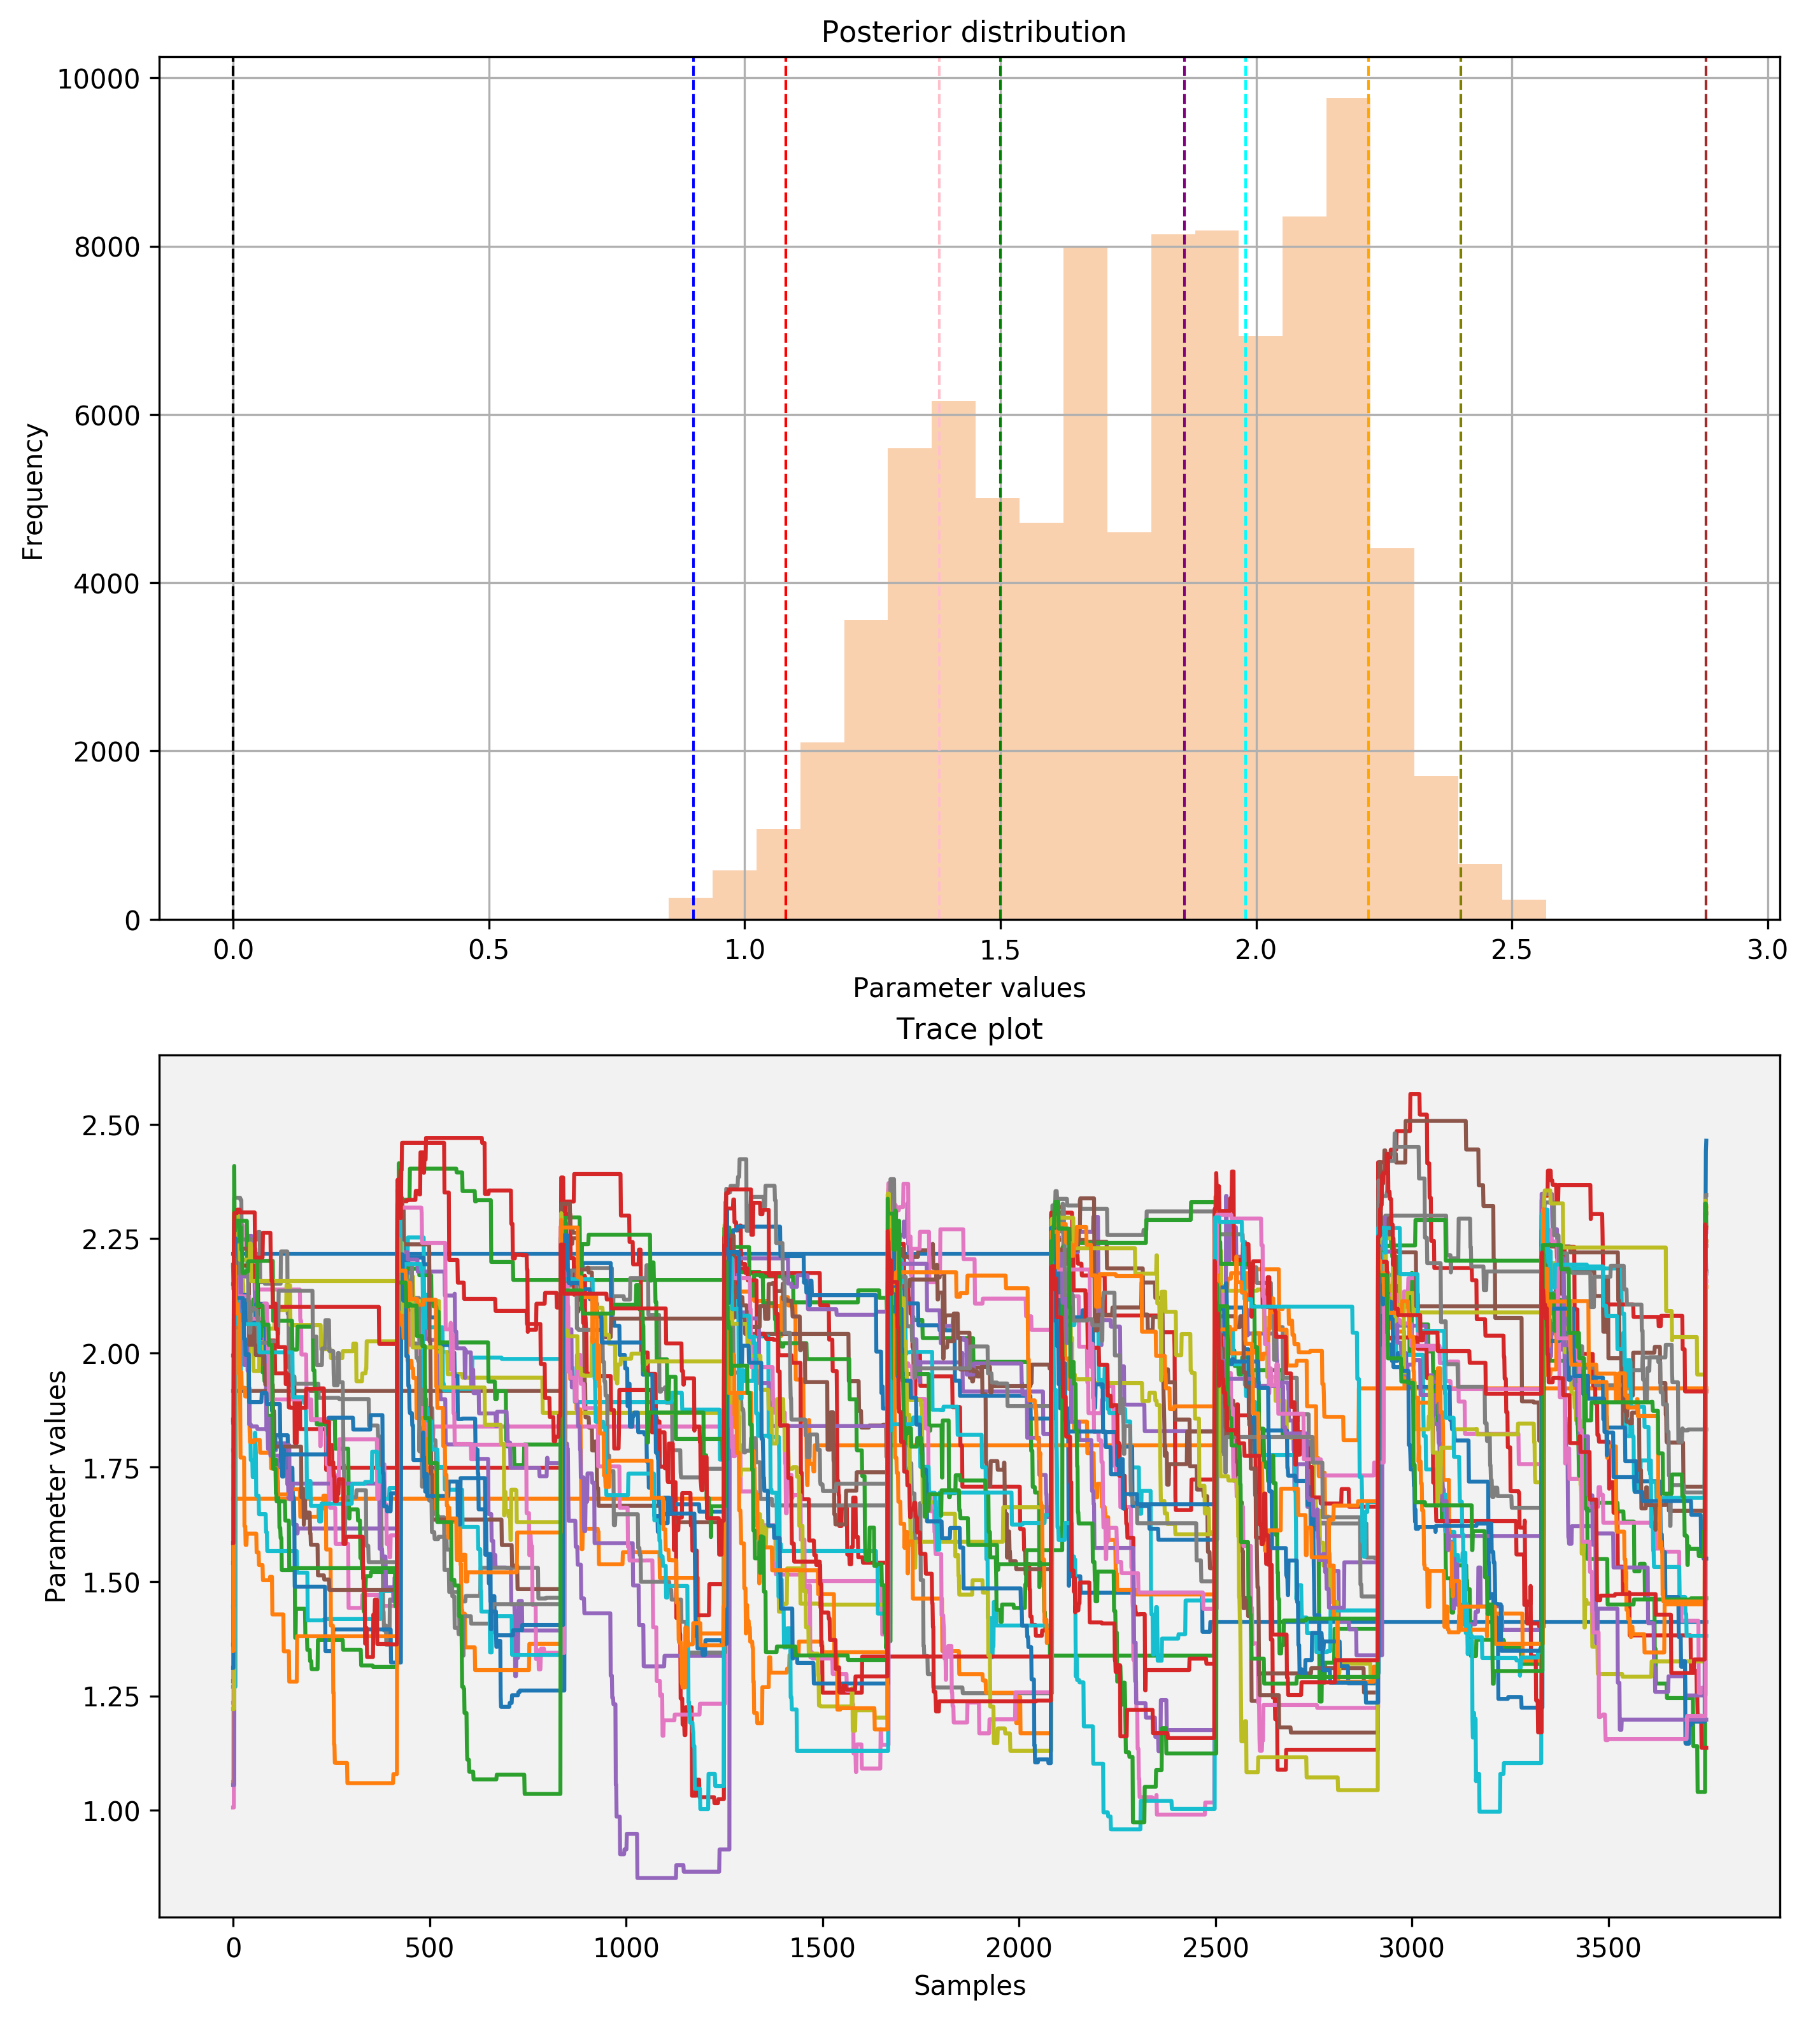
\includegraphics[width=70mm]{etopo_fast/pos_distri_0_pos_.png}}
       \subfigure[Etopo-short erodibility distribution]{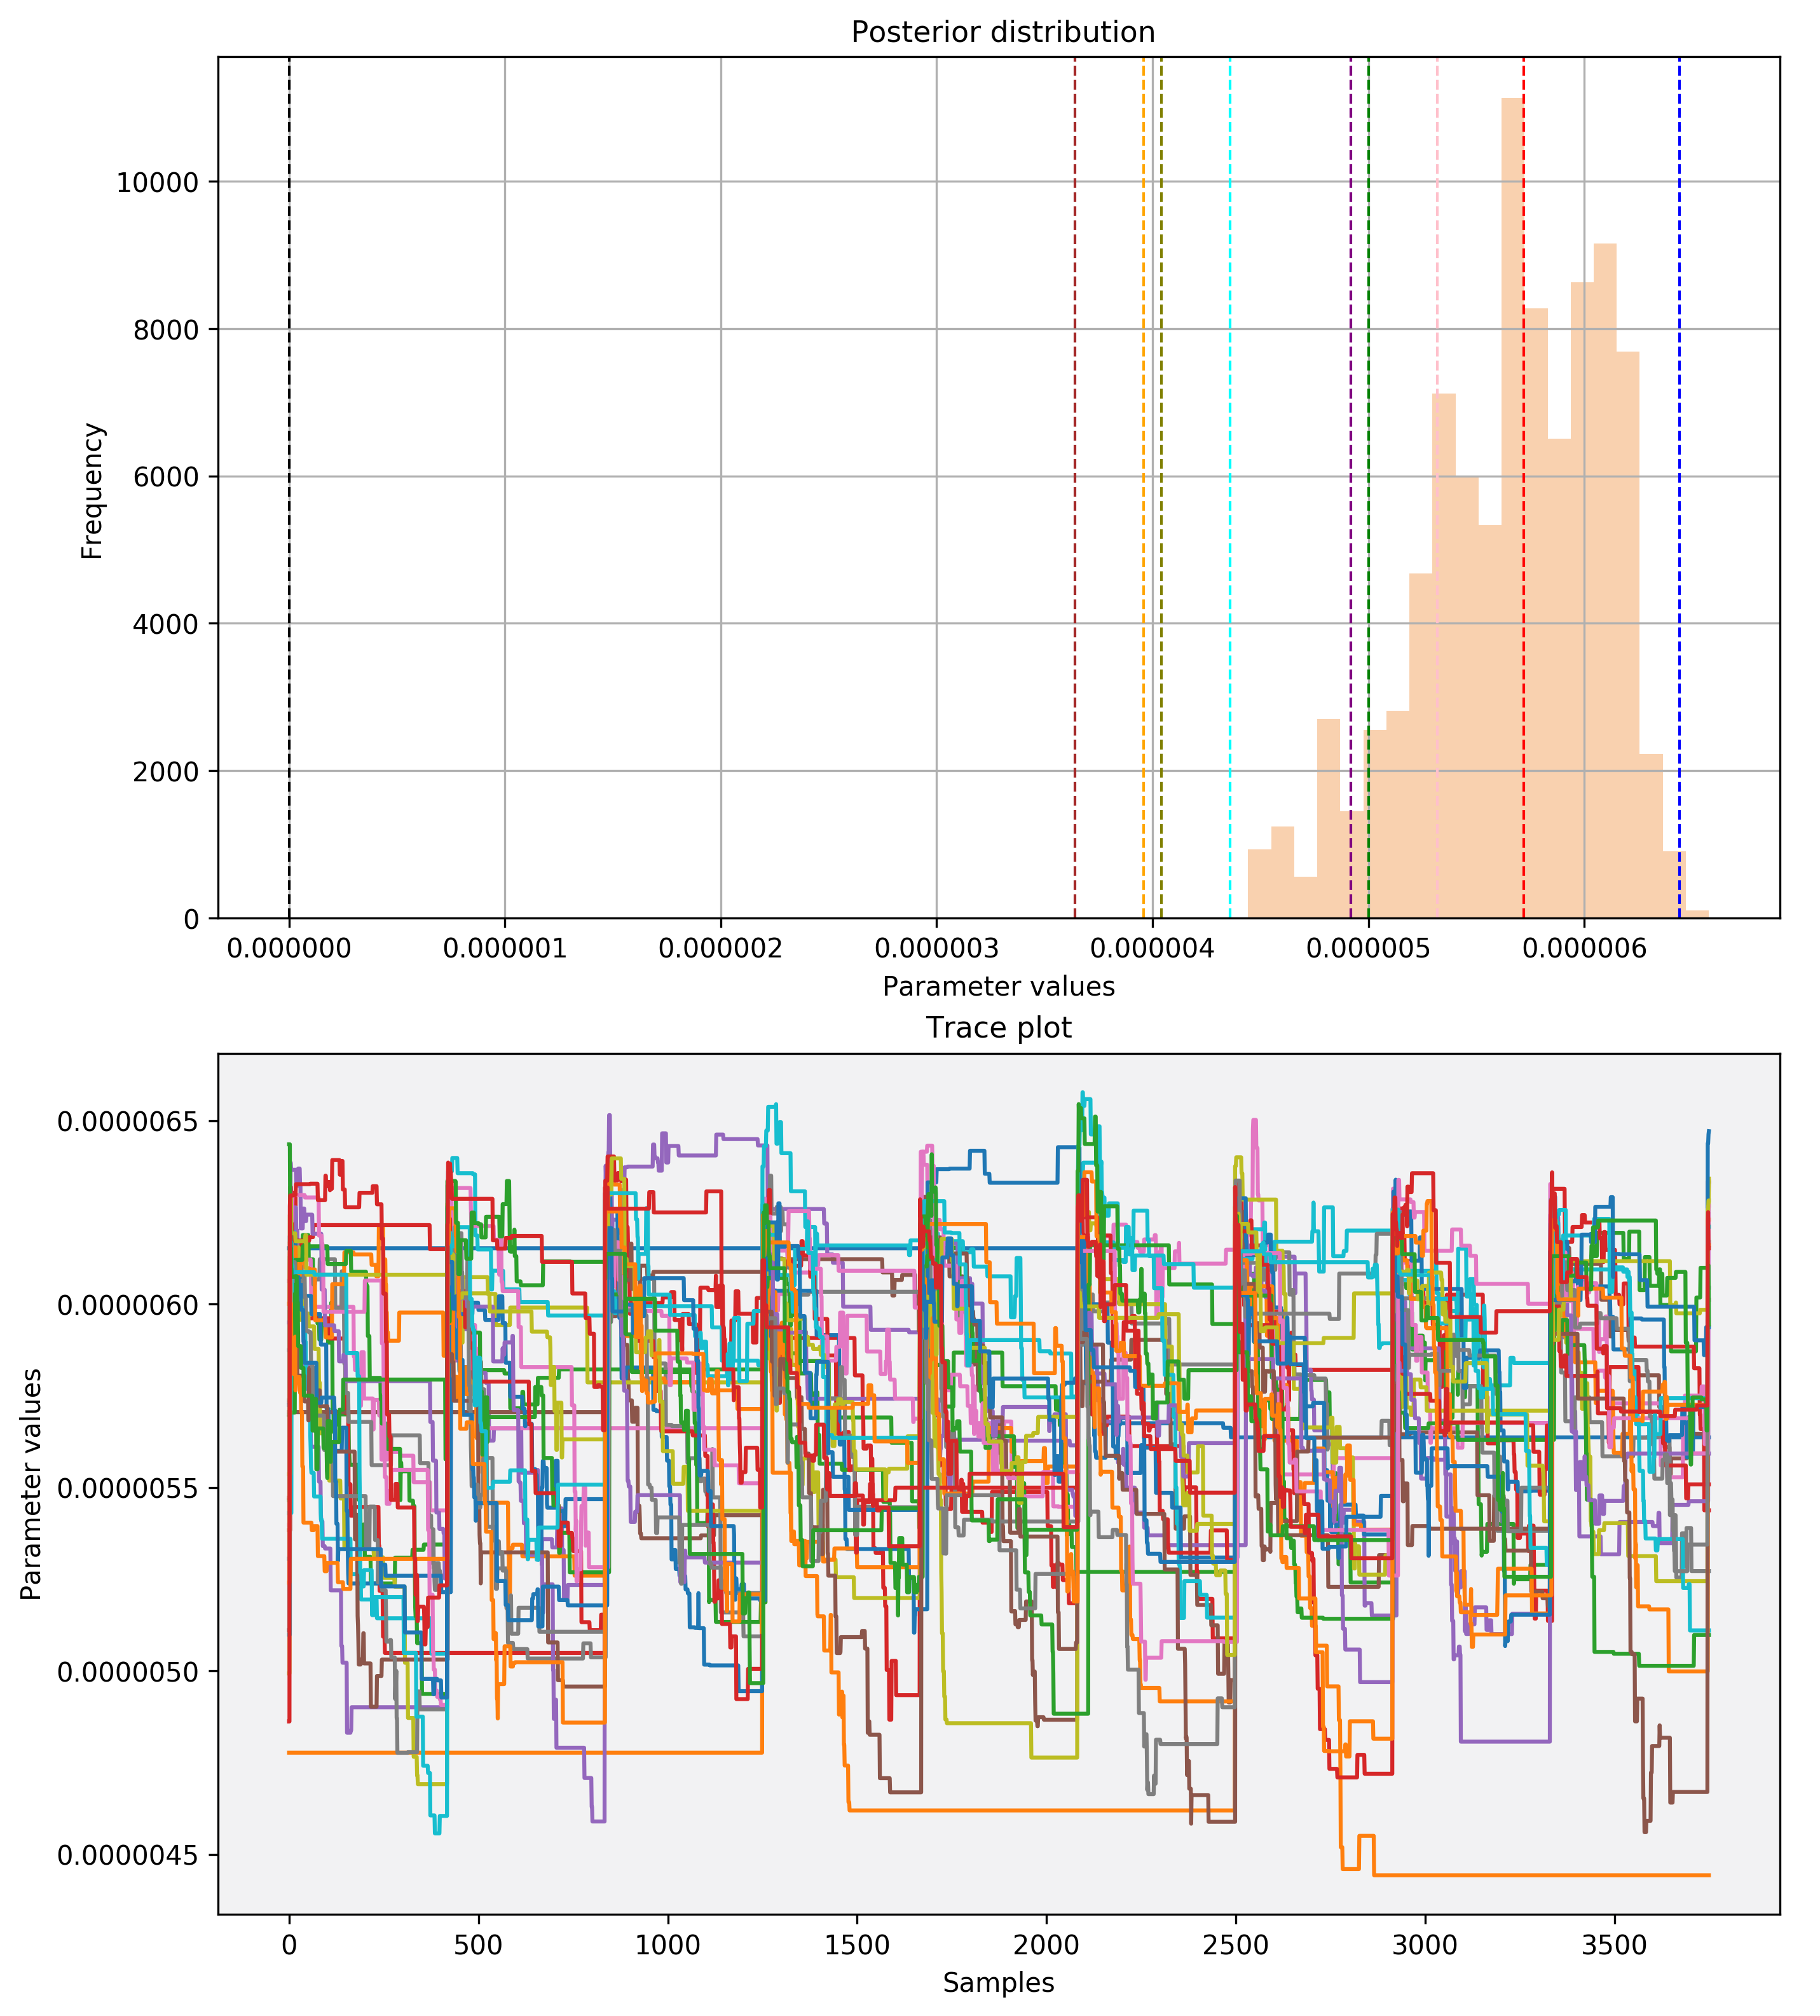
\includegraphics[width=70mm]{etopo_fast/pos_distri_1_pos_.png}}\\
       \subfigure[Etopo-short m distribution]{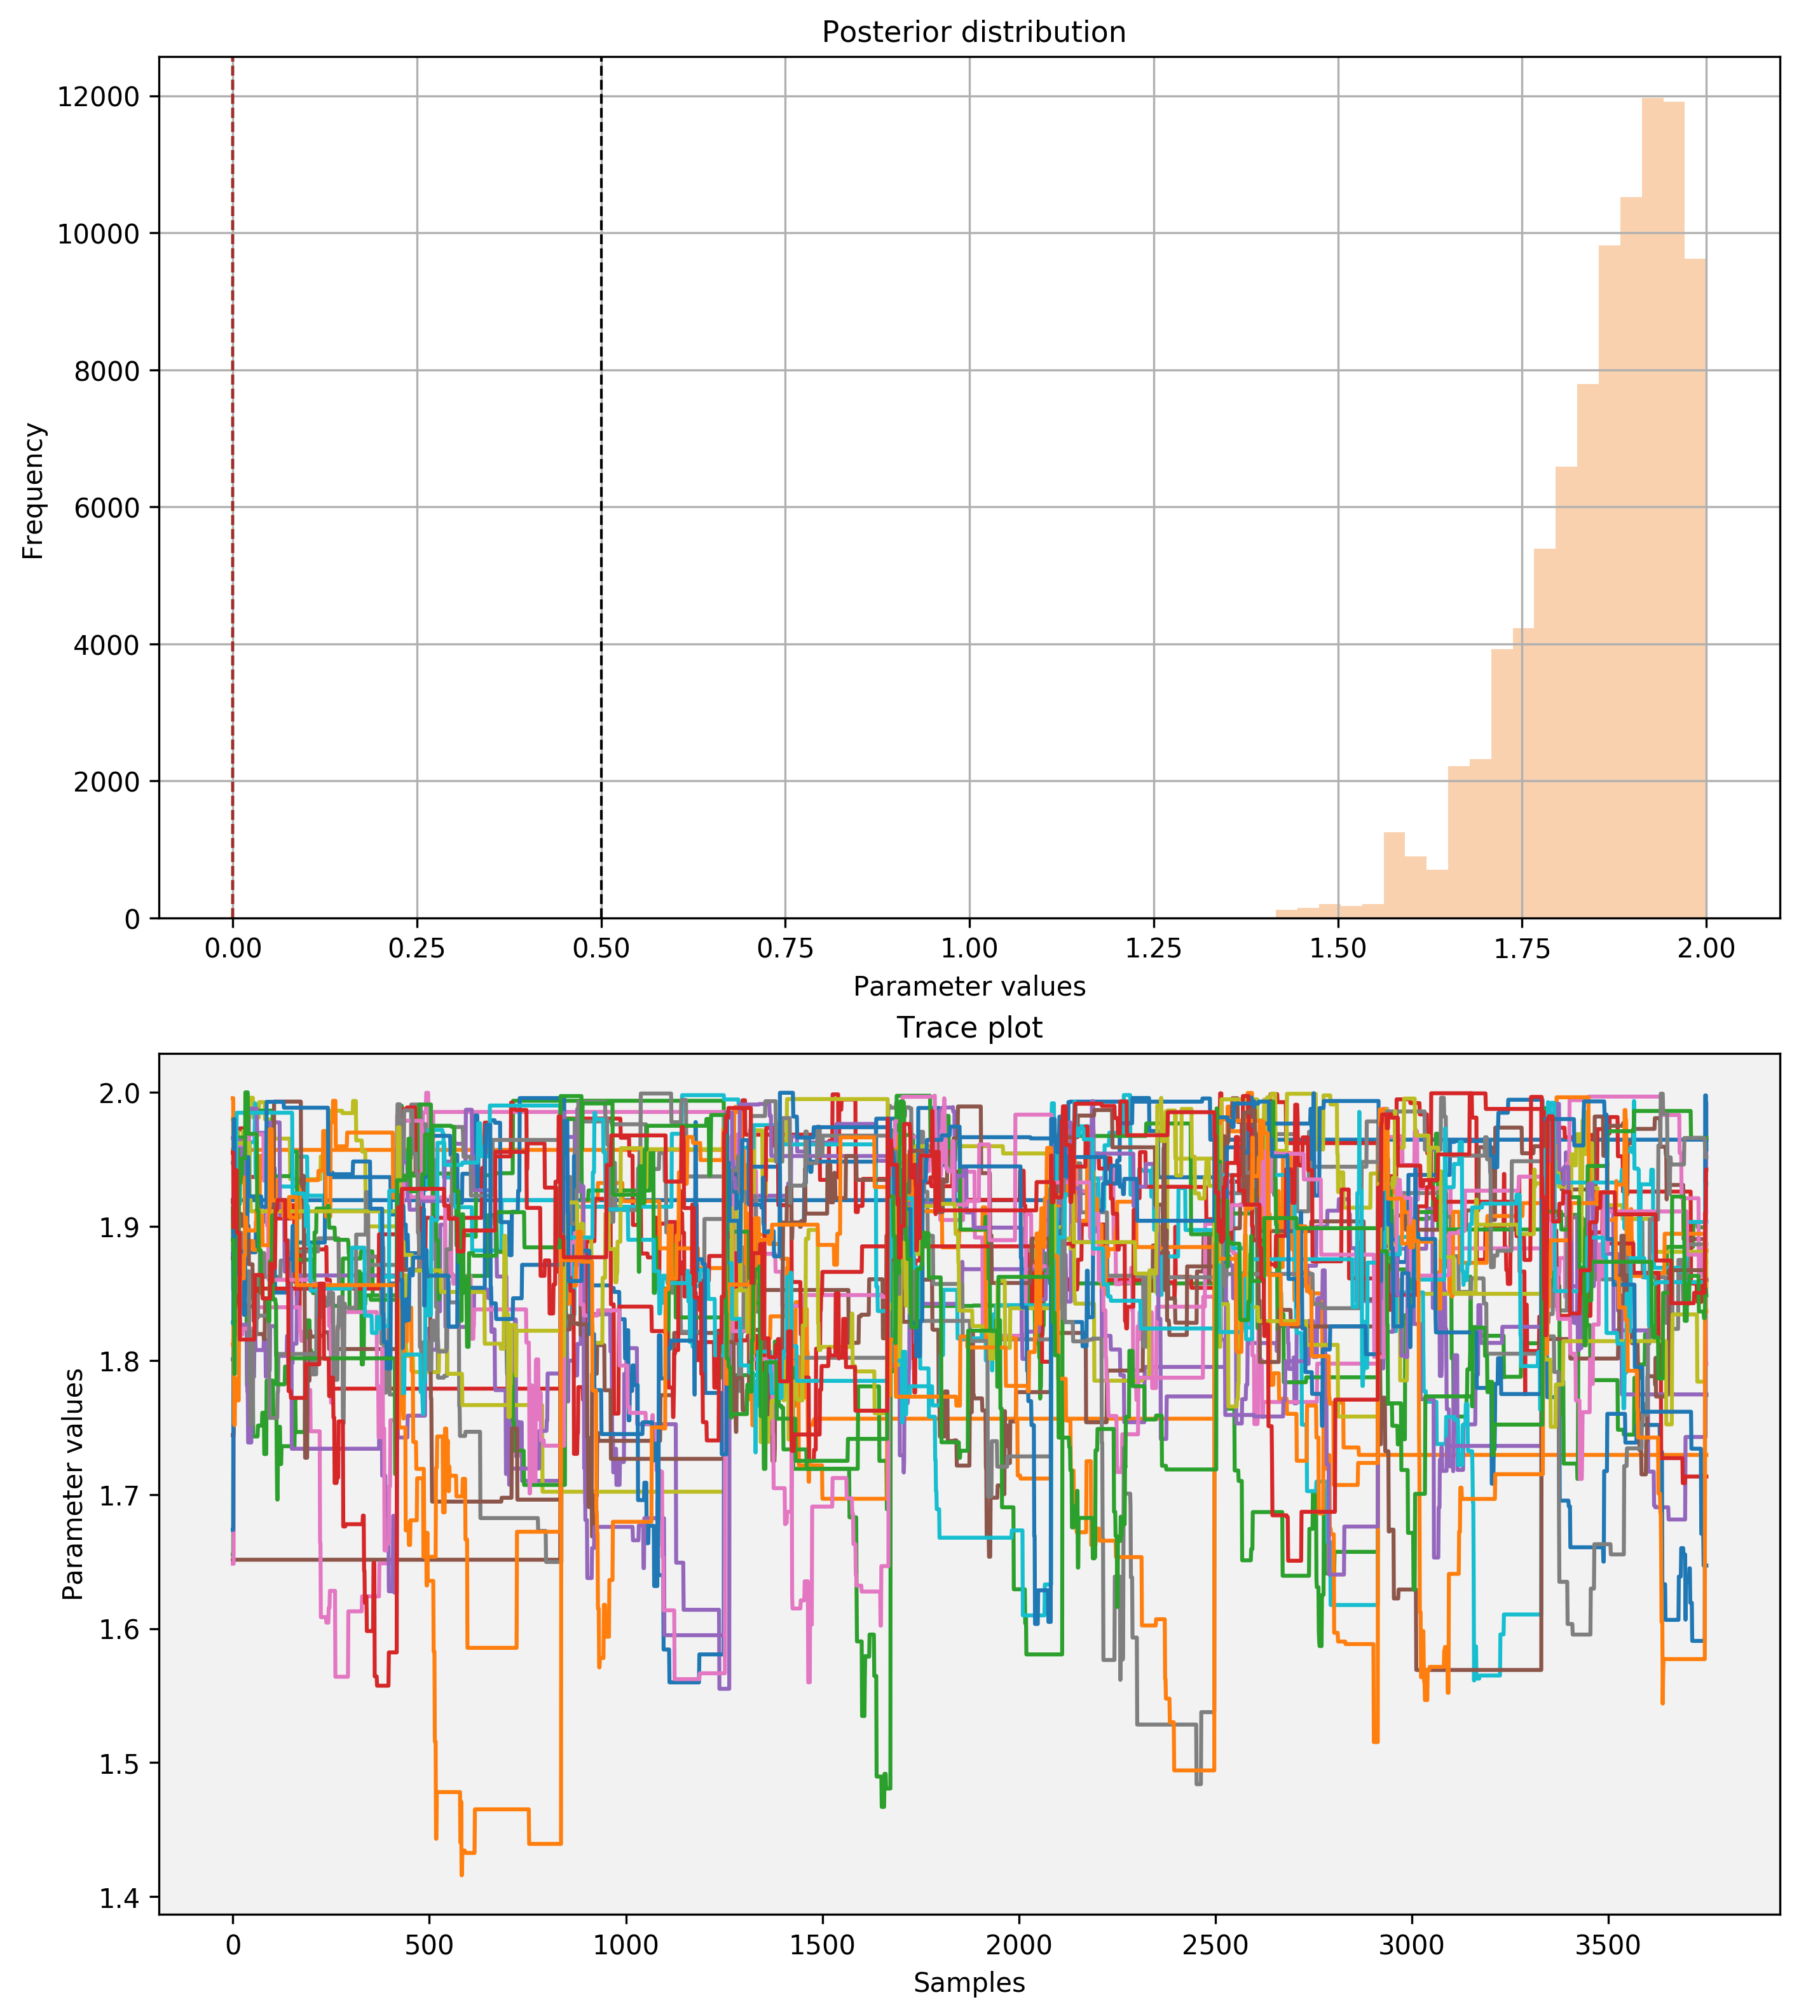
\includegraphics[width=70mm]{etopo_fast/pos_distri_2_pos_.png}}
       \subfigure[Etopo-short c-surface distribution]{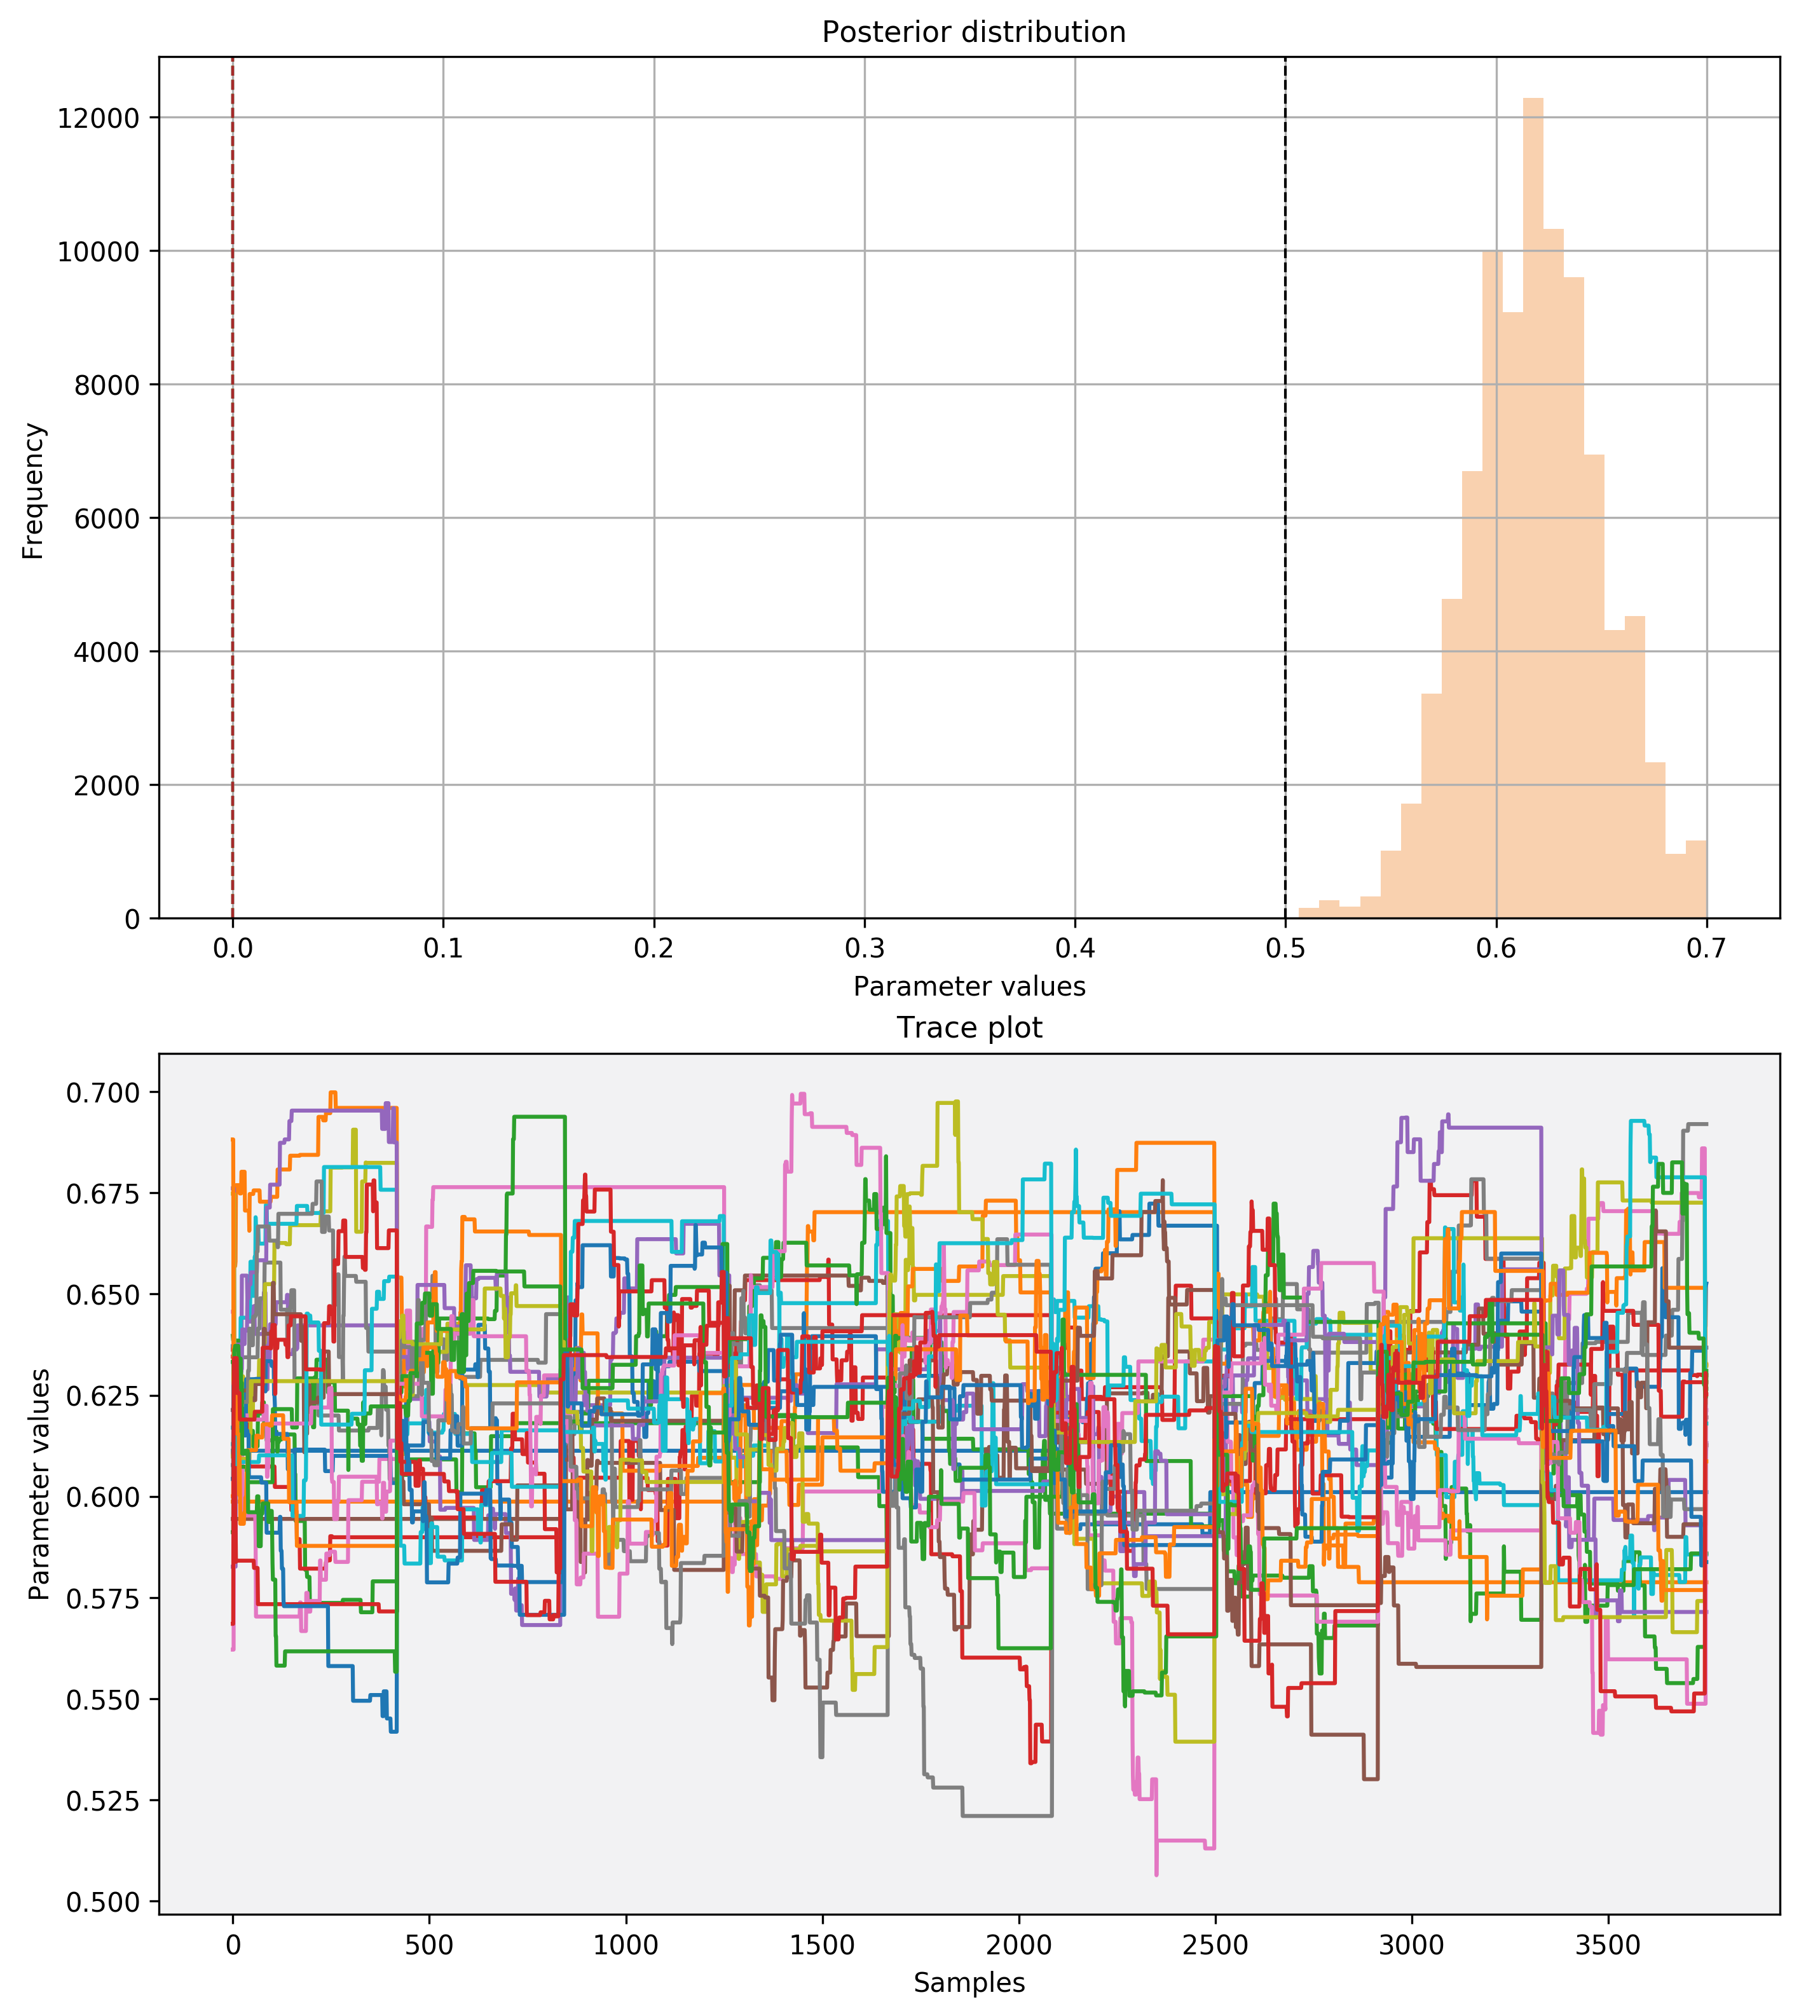
\includegraphics[width=70mm]{etopo_fast/pos_distri_5_pos_.png}}\\

     \end{tabular}
     \caption{Etopo-short: Posterior distribution of rainfall, erodibility, m and c-surface}
  \label{fig:etopo_fast_cmarine}
}
 \end{figure*}

 
 
  %-----------------------------------
  % eTopo
 %-----------------------------------

 \begin{figure*}[htb!]
{
\centering
     \begin{tabular}{cc} 
       \subfigure[Elevation cross-section along x-axis]{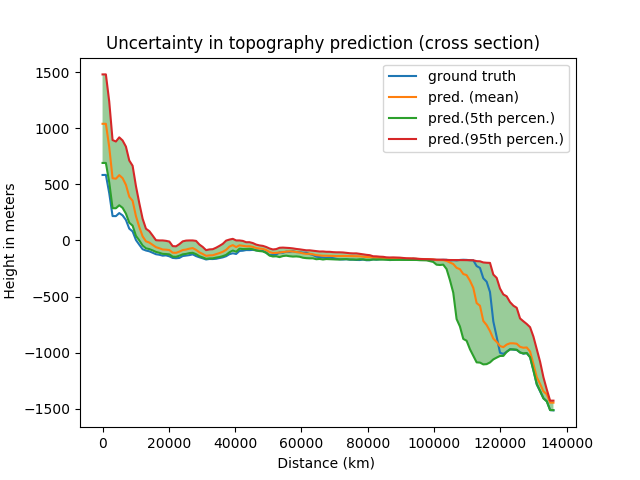
\includegraphics[width=70mm]{etopo/x_ymid_opt.png}} 
       \subfigure[Elevation cross-section along y-axis]{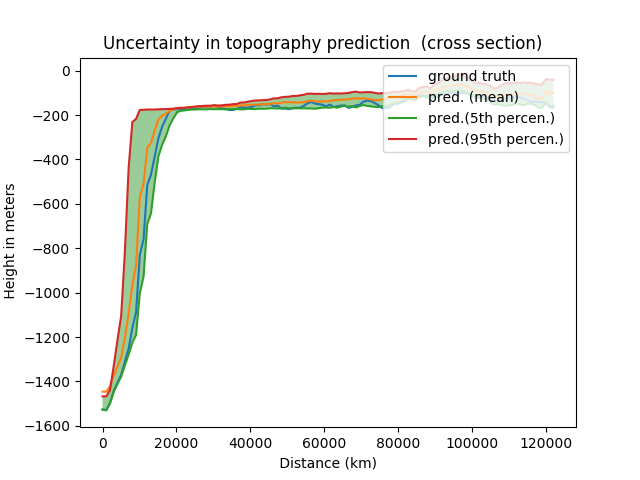
\includegraphics[width=70mm]{etopo/y_xmid_opt.png}}\\
     \end{tabular}
     \caption{eTopo: Elevation cross-section taken at mid-point along x-axis and y-axis }
  \label{fig:etopo_cross}
}
 \end{figure*}
 
 
 %-----------------------------------
 
\begin{figure*}[htb!]
{
\centering
    \begin{tabular}{cc} 
      \subfigure[eTopo erosion-deposition after 25 \% evolution time ]{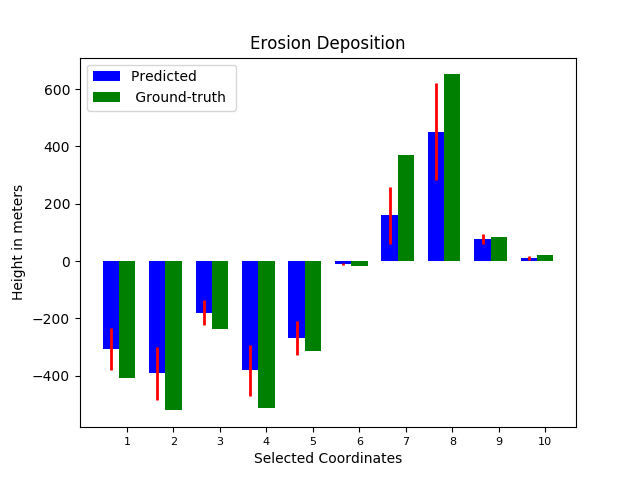
\includegraphics[width=80mm]{etopo/pos_erodep_250000.png}} 
      \subfigure[eTopo erosion-deposition  after 50 \% evolution time]{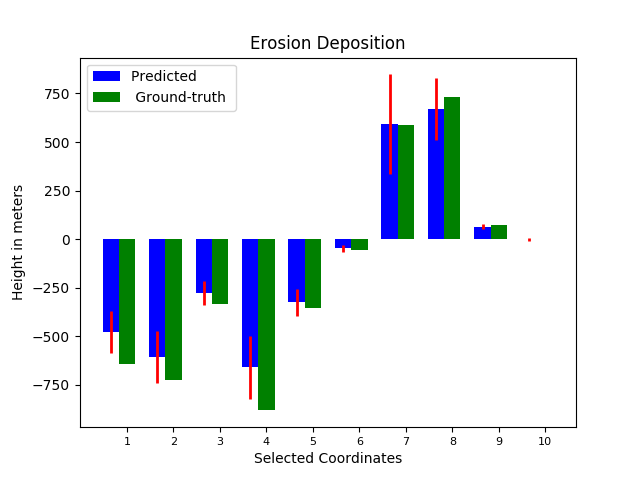
\includegraphics[width=80mm]{etopo/pos_erodep_500000.png}}\\ 
       \subfigure[eTopo erosion-deposition after 75 \% evolution time ]{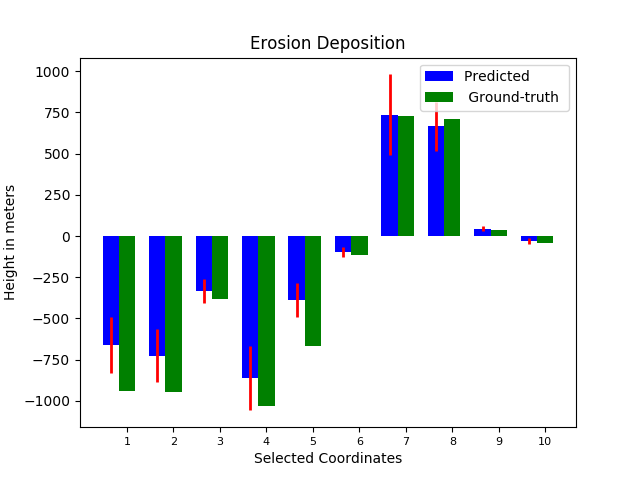
\includegraphics[width=80mm]{etopo/pos_erodep_750000.png}} 
      \subfigure[eTopo erosion-deposition  after 100 \% evolution time]{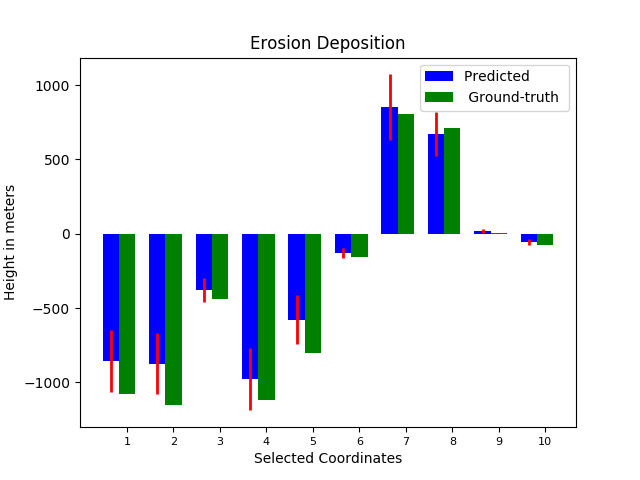
\includegraphics[width=80mm]{etopo/pos_erodep_1000000.png}}\\
    \end{tabular}
    \caption{eTopo erosion-deposition}
 \label{fig:etopo_erodep}
}
\end{figure*}


%----------------------------------

\begin{figure*}[htb!]
{
\centering
    \begin{tabular}{cc} 
      \subfigure[eTopo rainfall distribution]{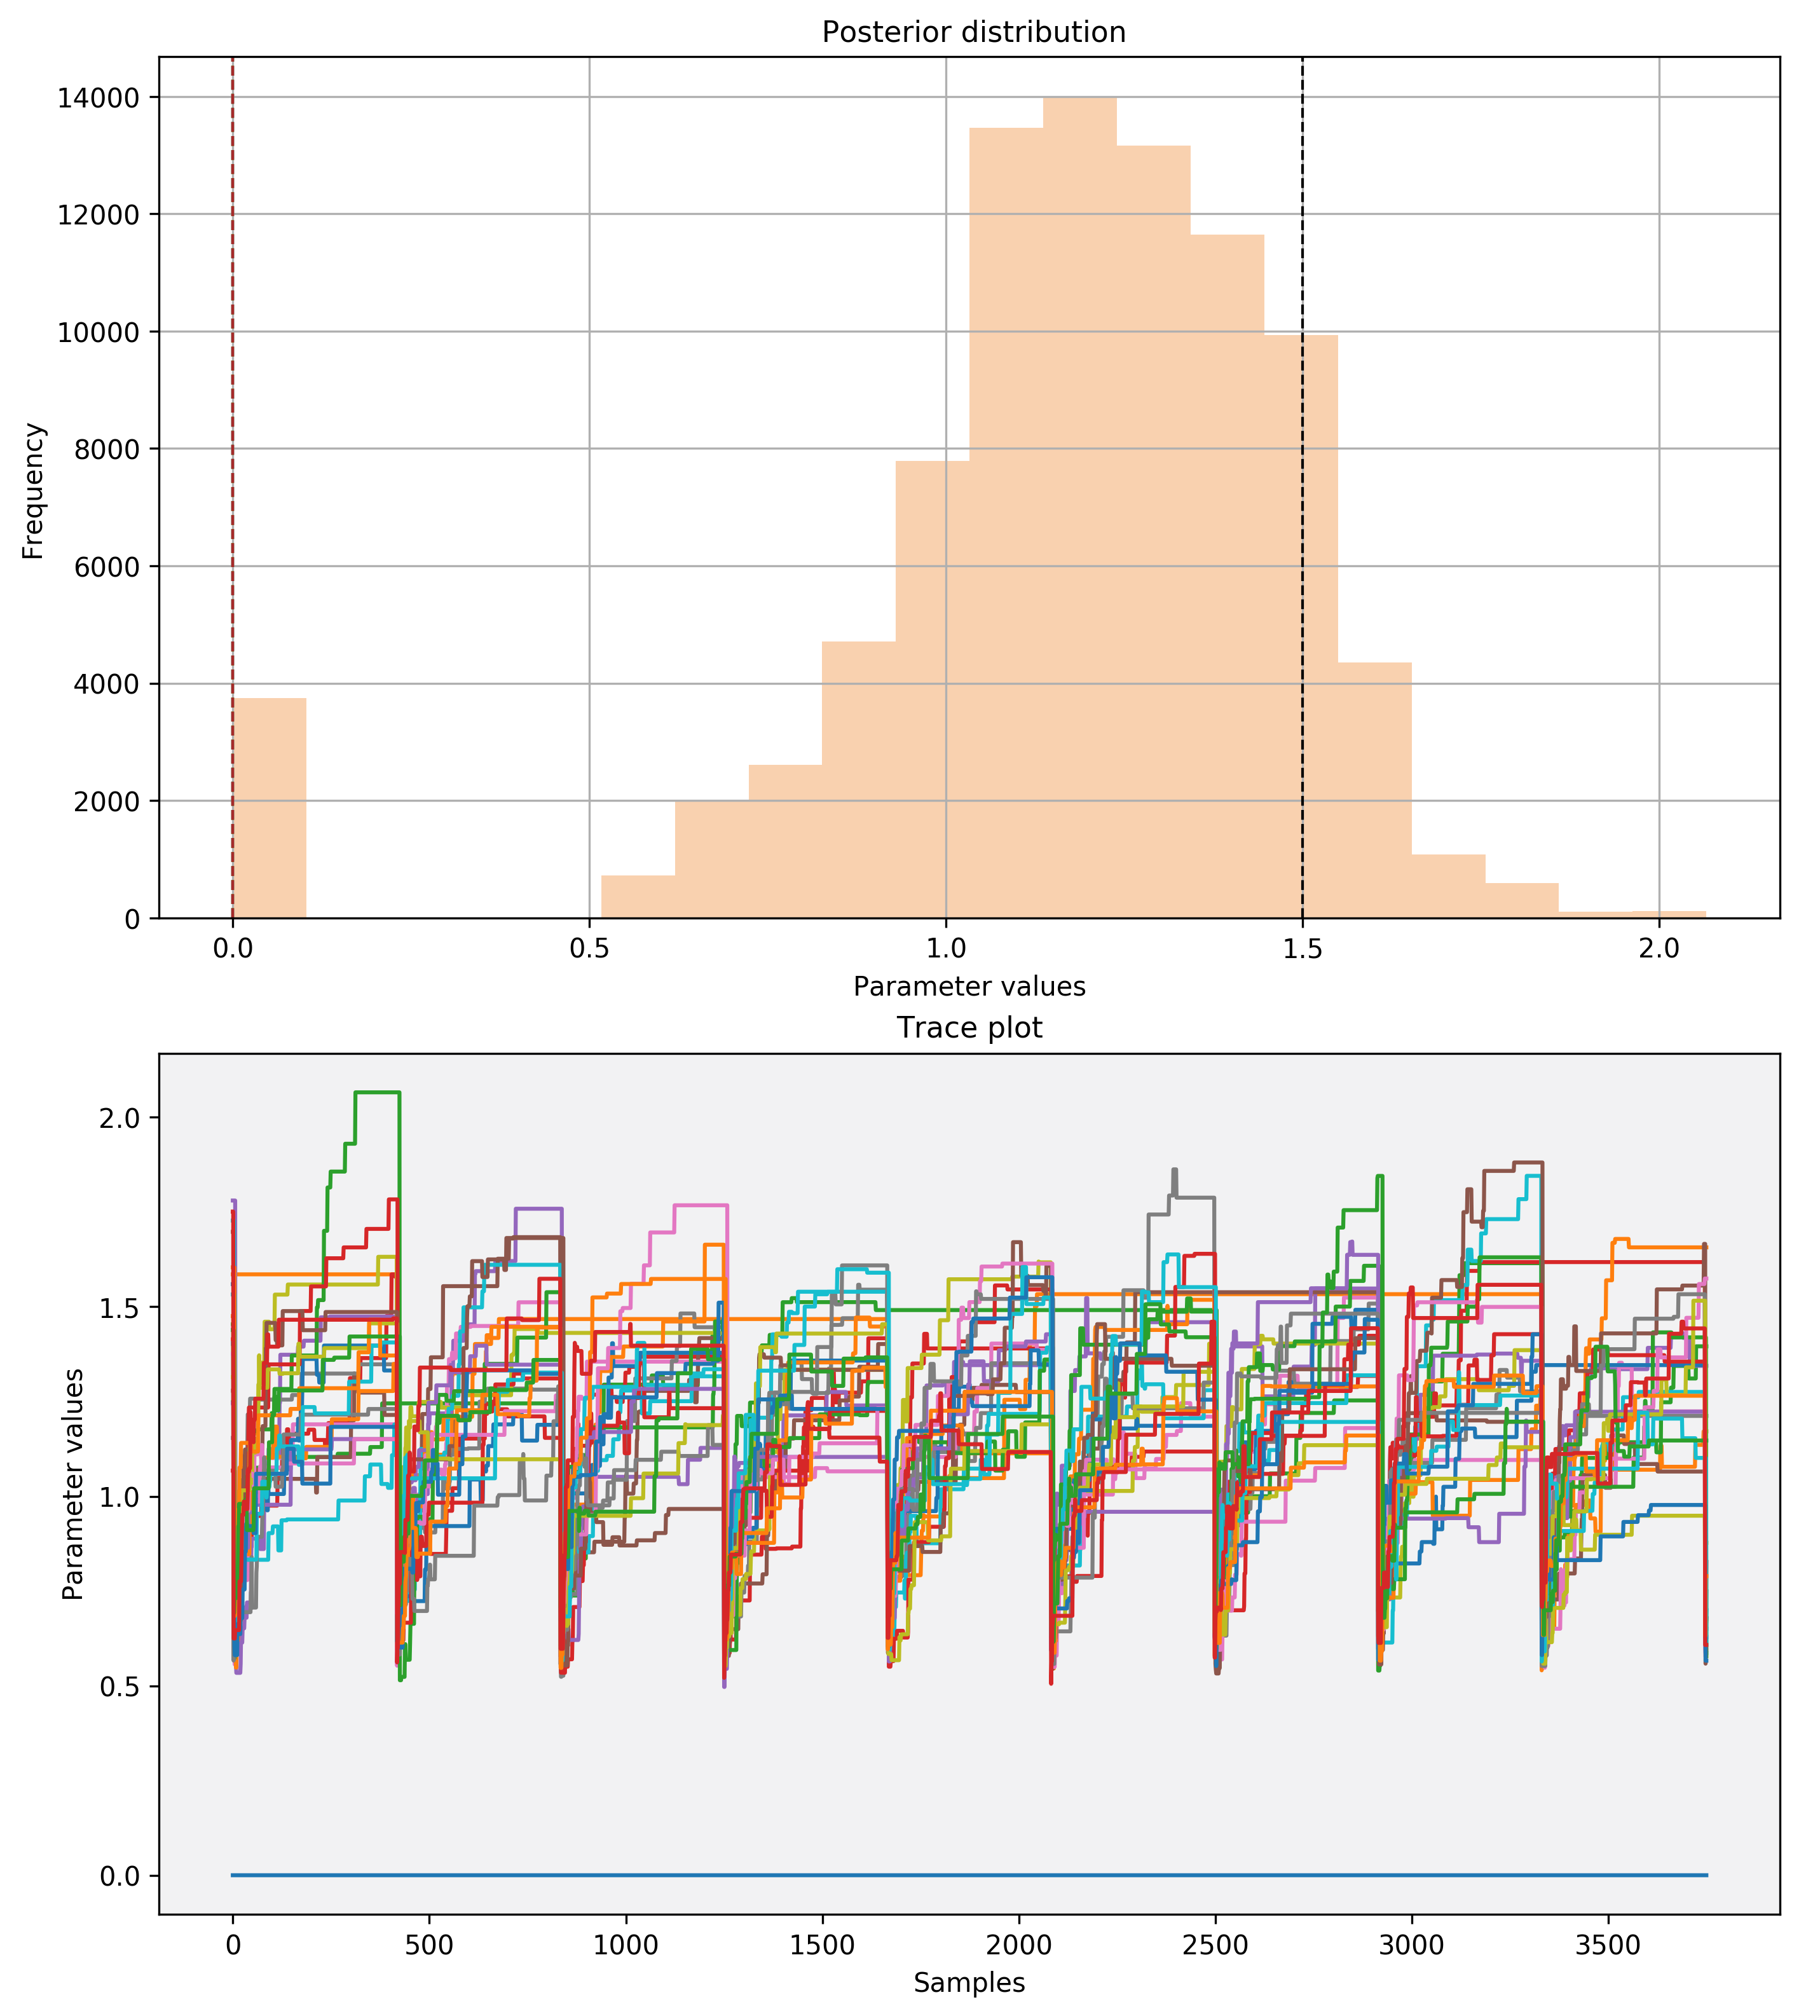
\includegraphics[width=70mm]{etopo/pos_distri_0_pos_.png}} 
      \subfigure[eTopo erodibility distribution]{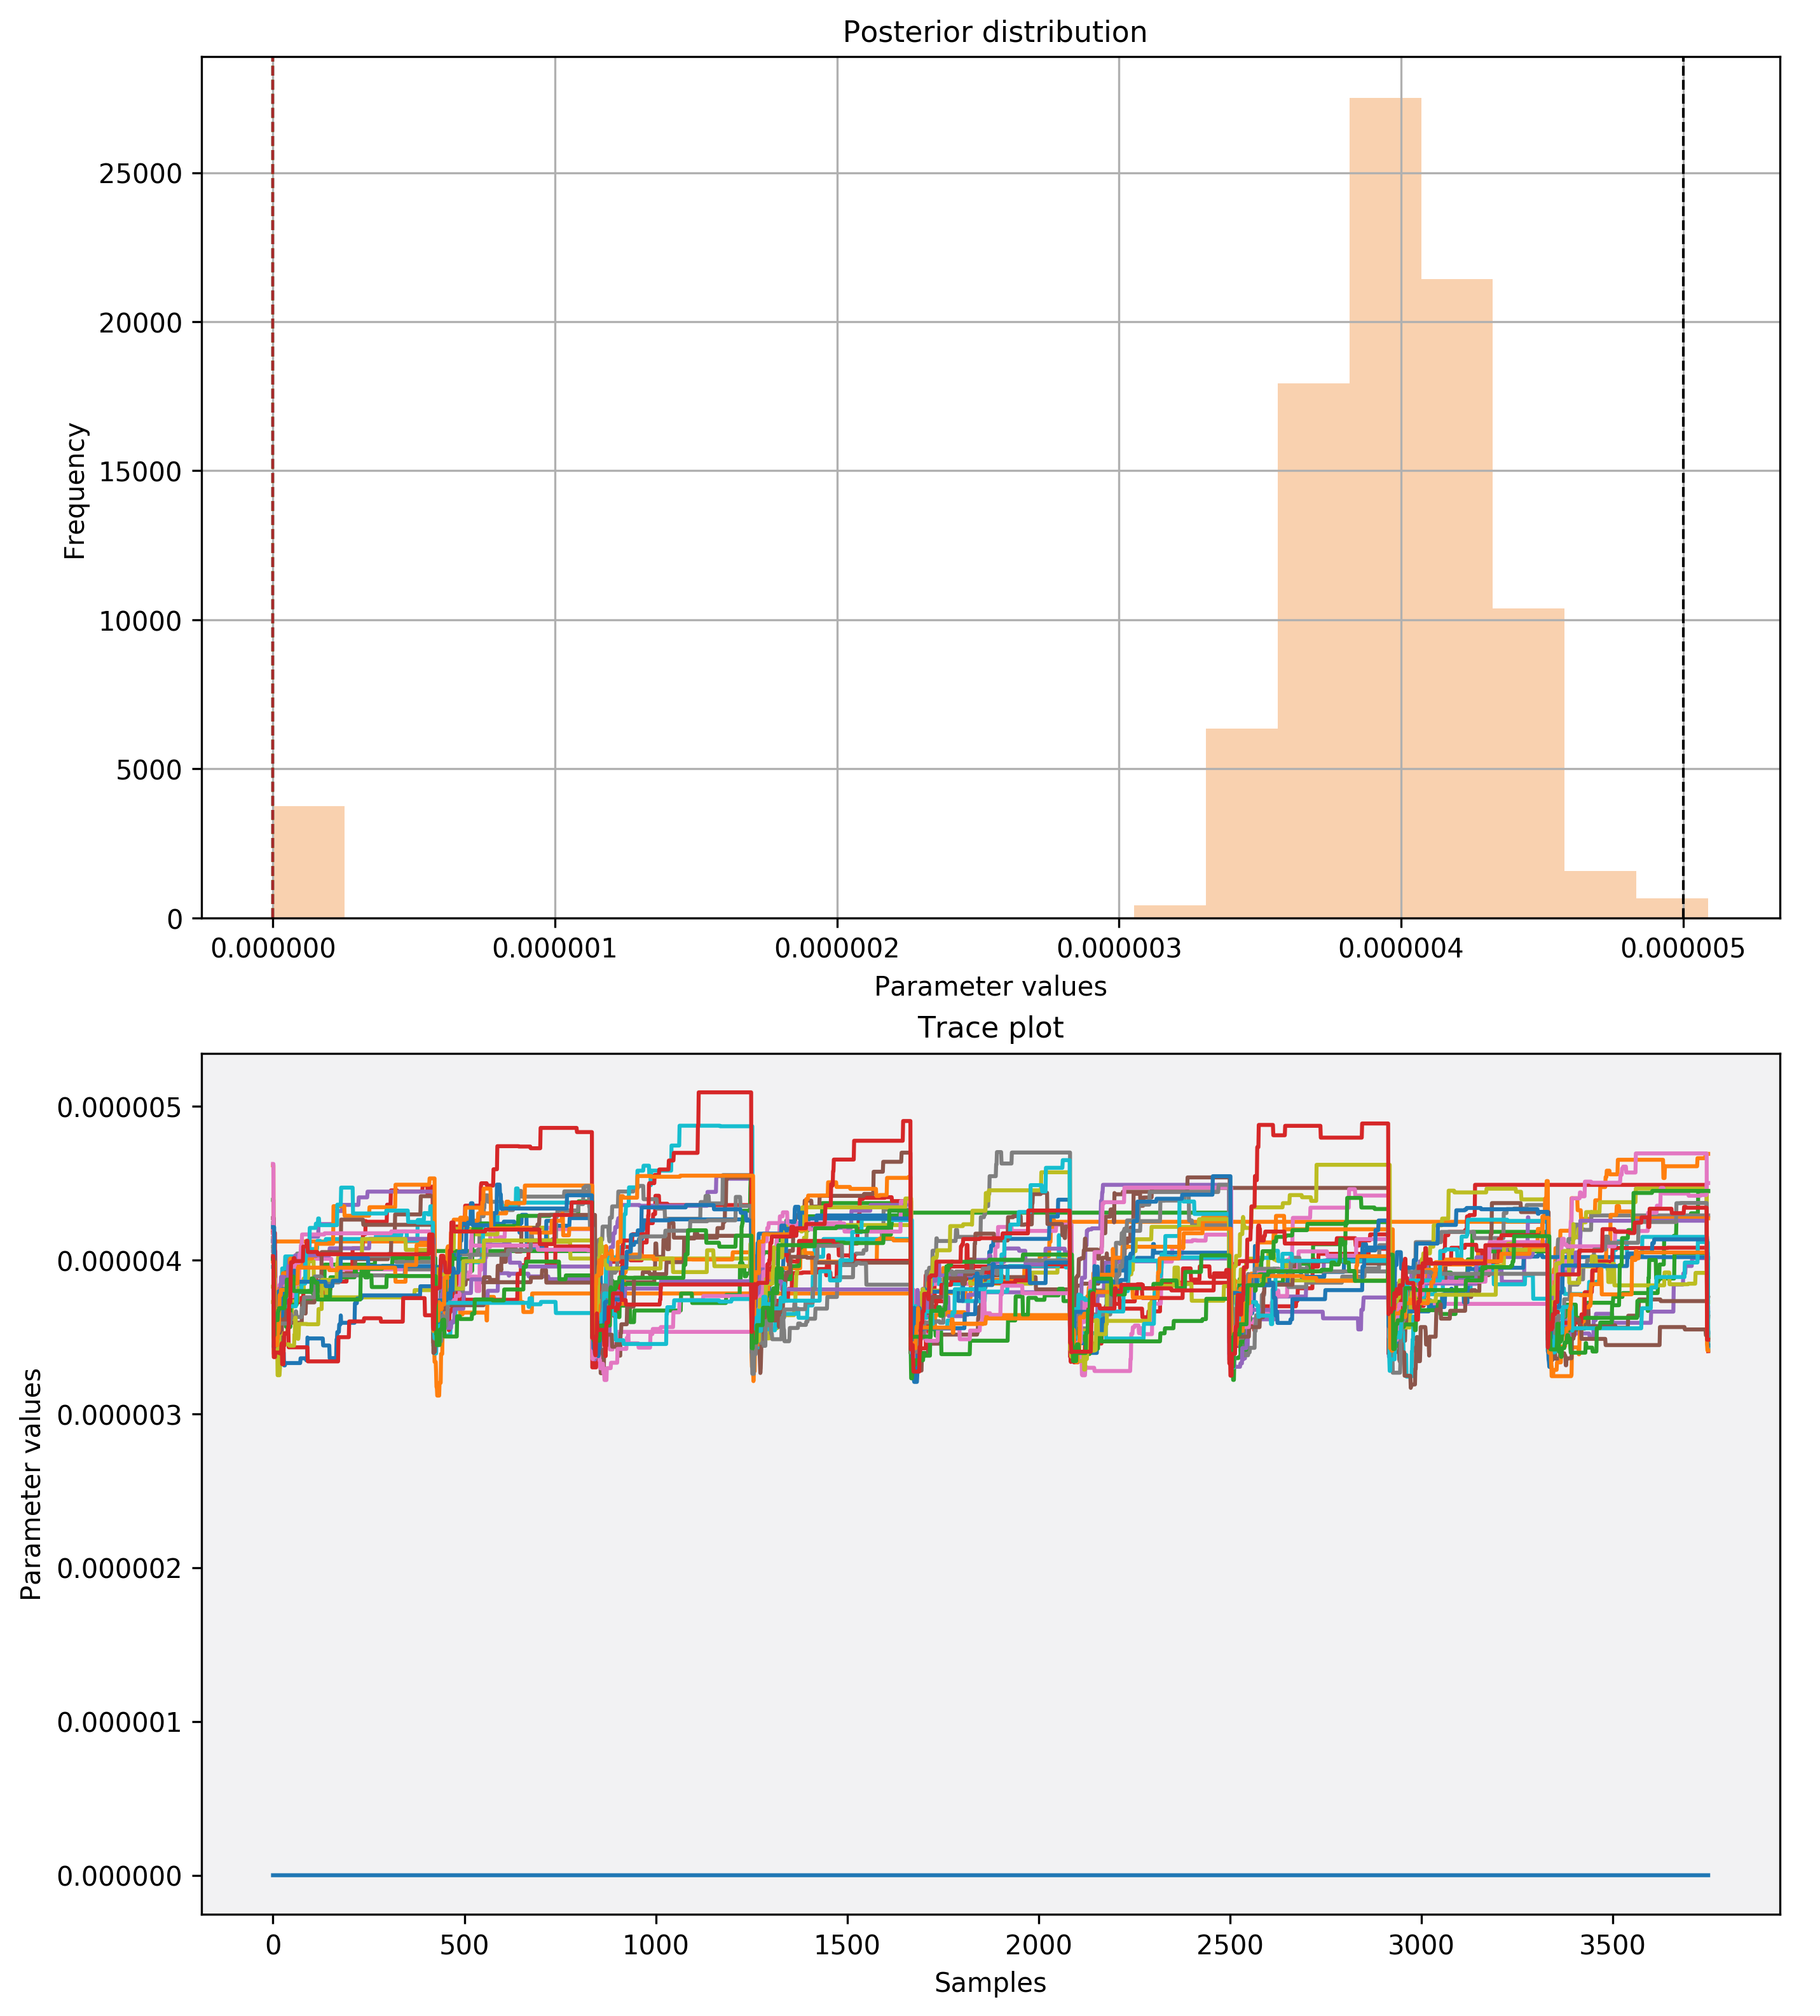
\includegraphics[width=70mm]{etopo/pos_distri_1_pos_.png}}\\
      \subfigure[eTopo m distribution]{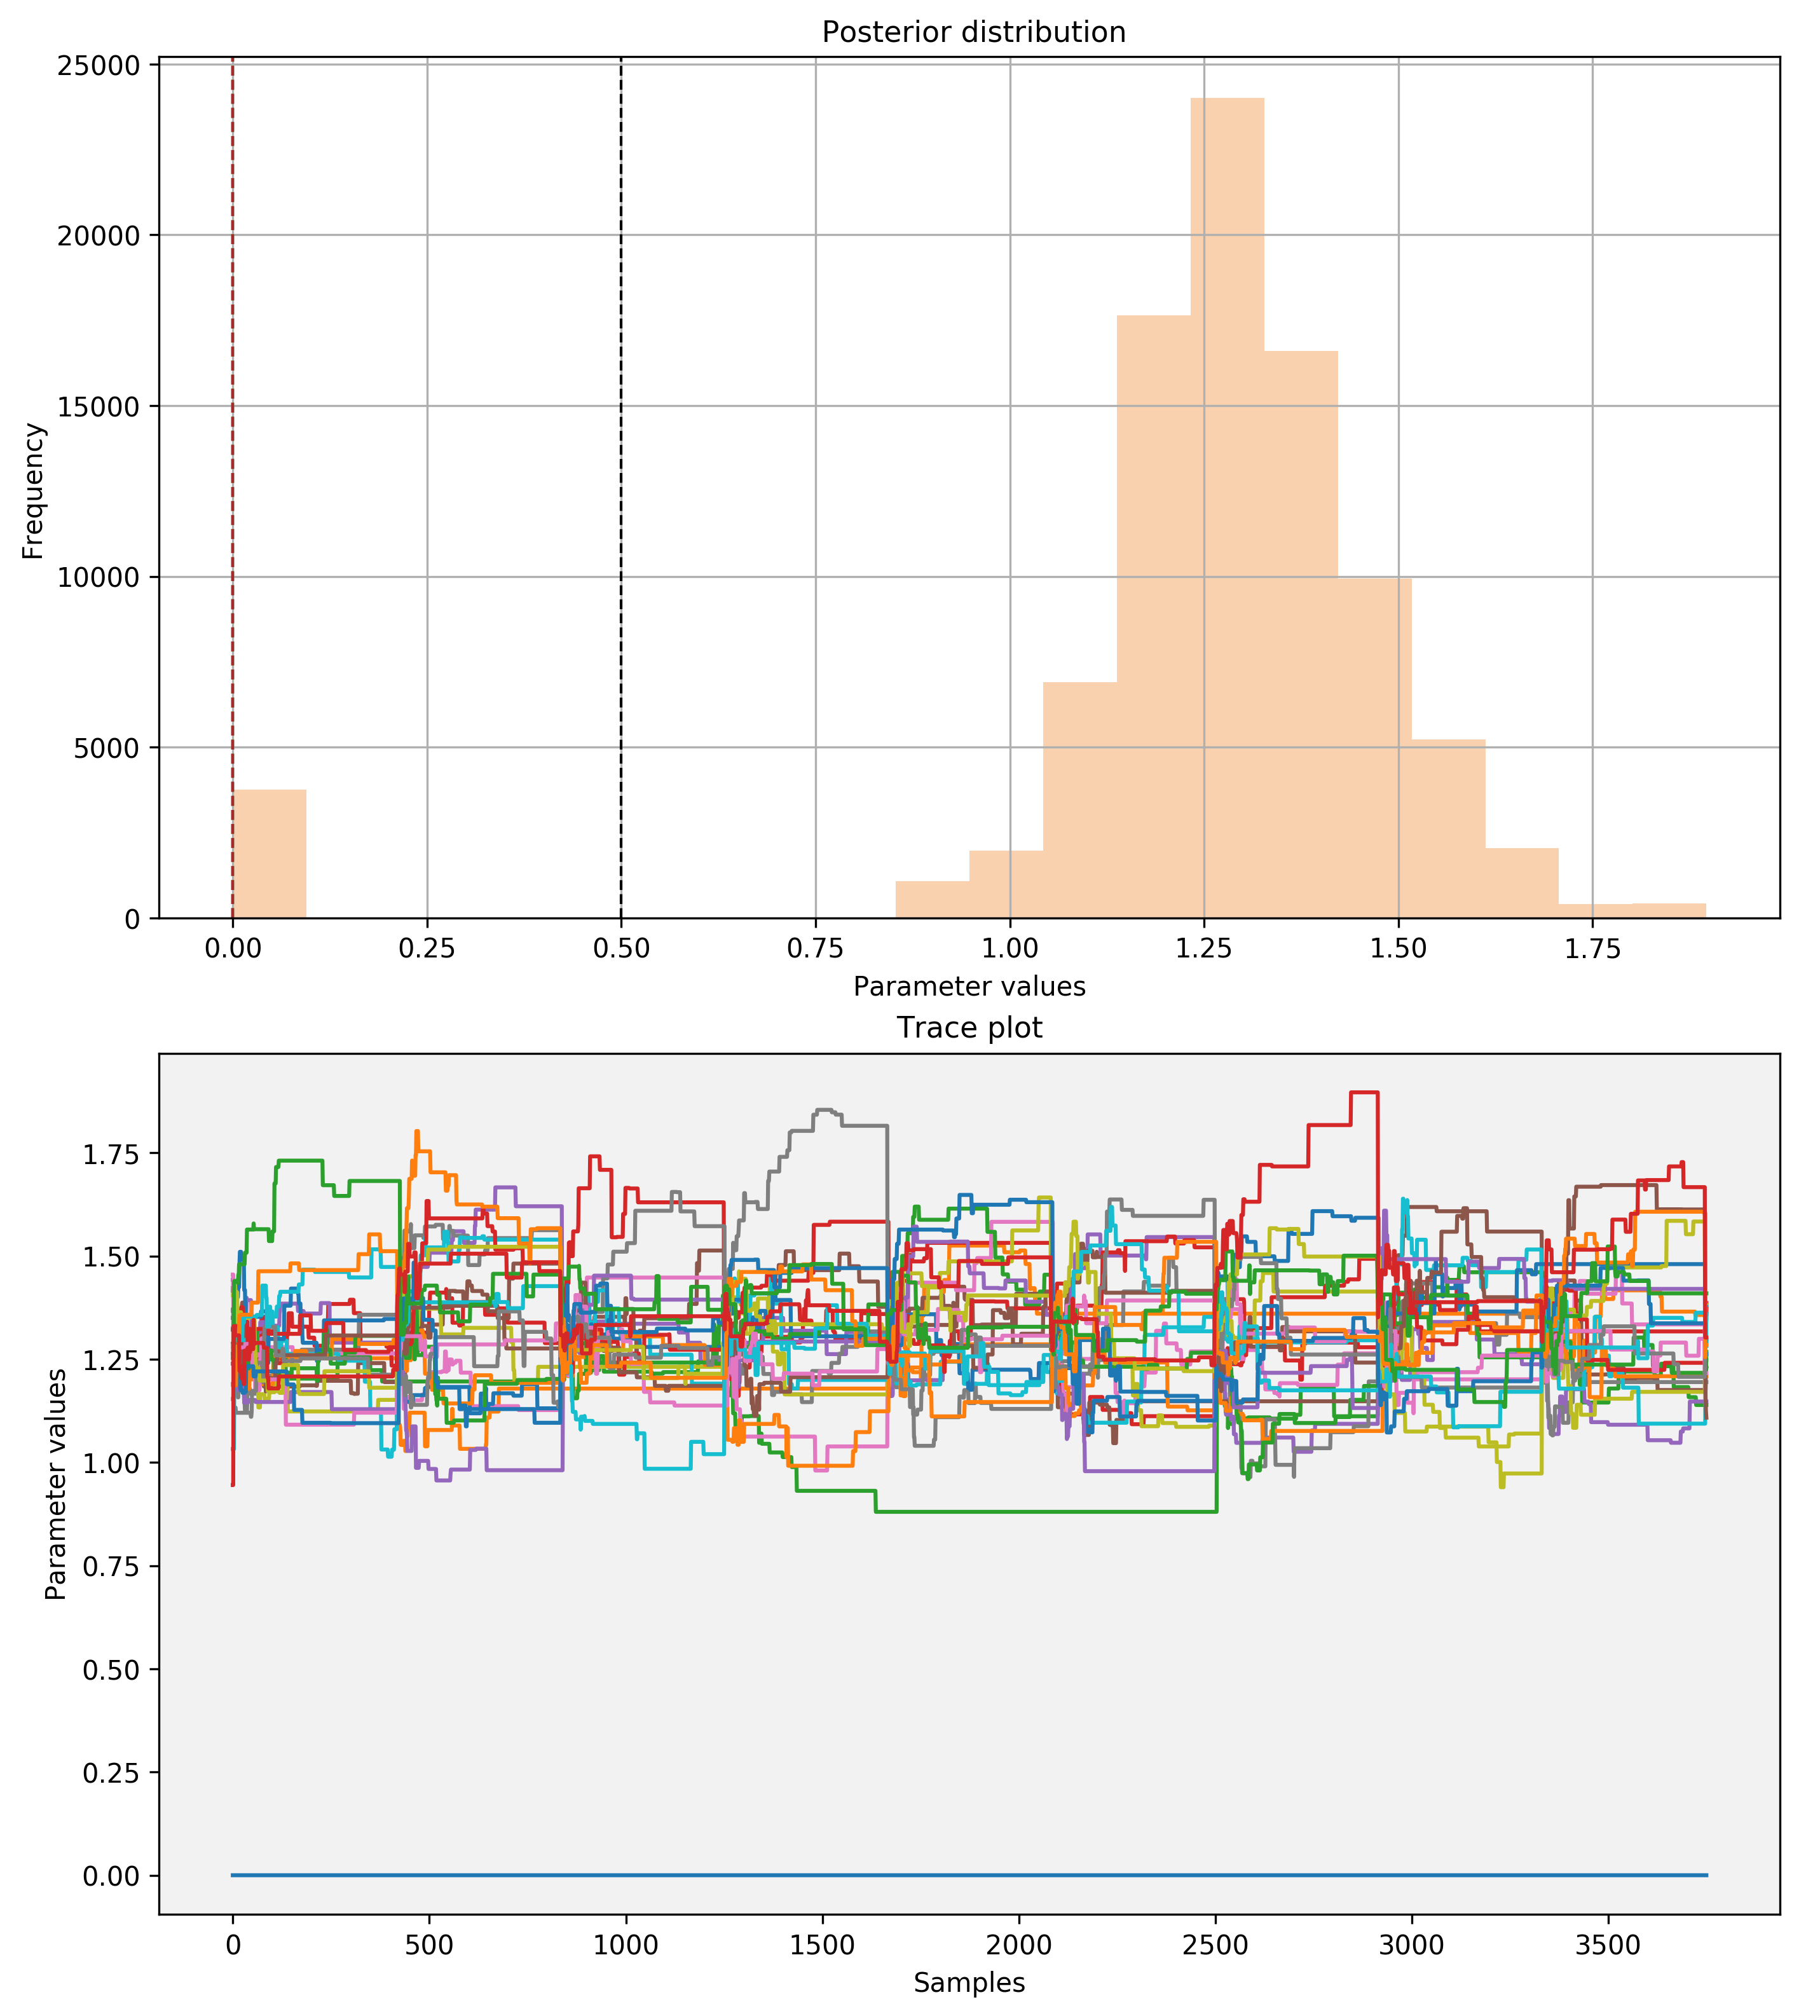
\includegraphics[width=70mm]{etopo/pos_distri_2_pos_.png}} 
      \subfigure[eTopo c-surface distribution]{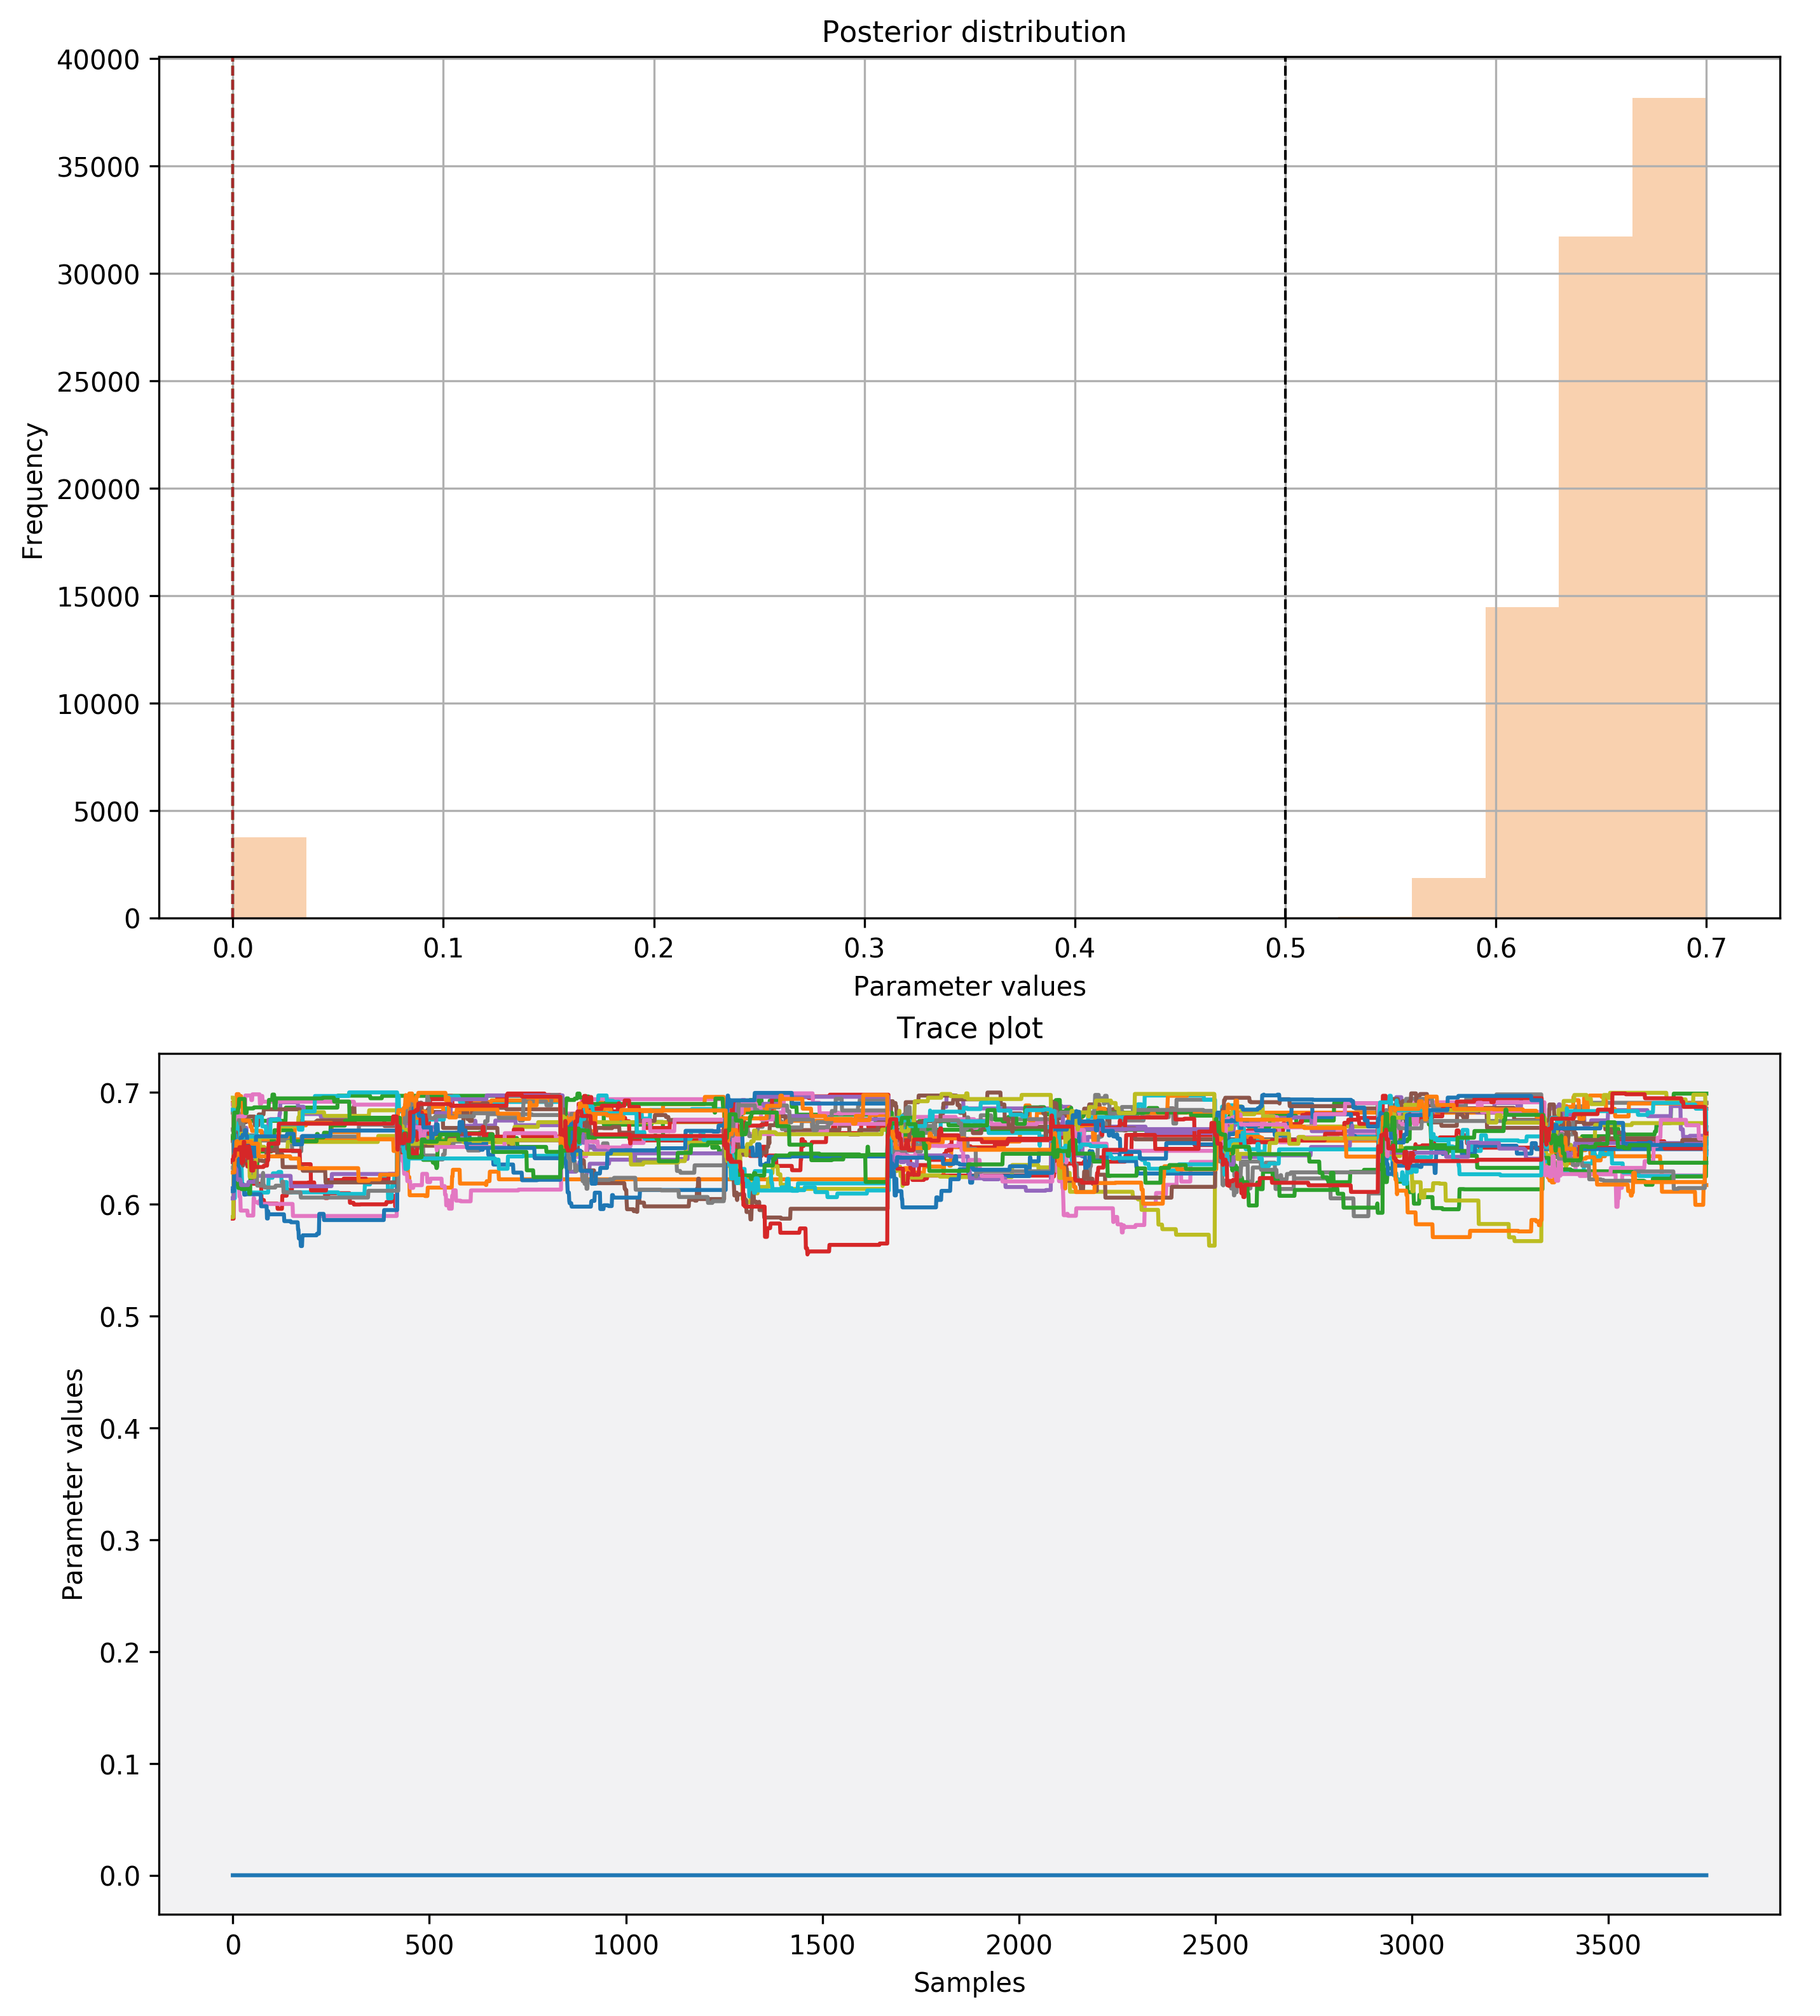
\includegraphics[width=70mm]{etopo/pos_distri_5_pos_.png}}\\
       
    \end{tabular}
    \caption{eTopo: Posterior distribution of rainfall, erodibility, m and c-surface}
 \label{fig:etopo_cmarine}
}
\end{figure*}

%----------------------------------
%----------------------------------


\begin{figure*}[htb!]
  \begin{center}
    \begin{tabular}{cc}
      \subfigure[Crater-short posterior  (rainfall, erodibility, m, n )]{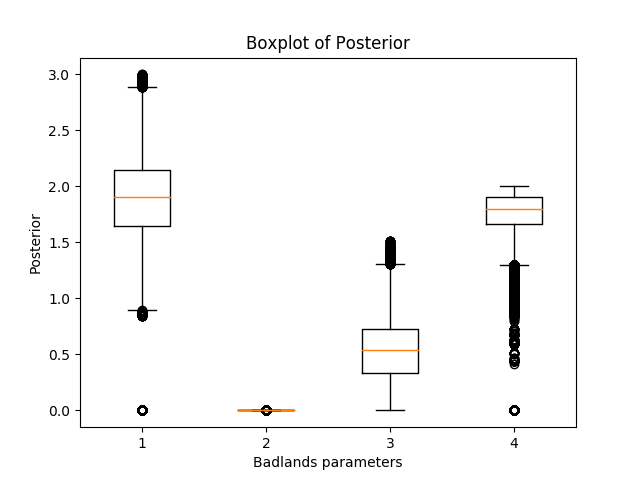
\includegraphics[width=75mm]{crater_fast/badlands_pos.png}}
      \subfigure[ Crater  posterior  (rainfall, erodibility, m, n )]{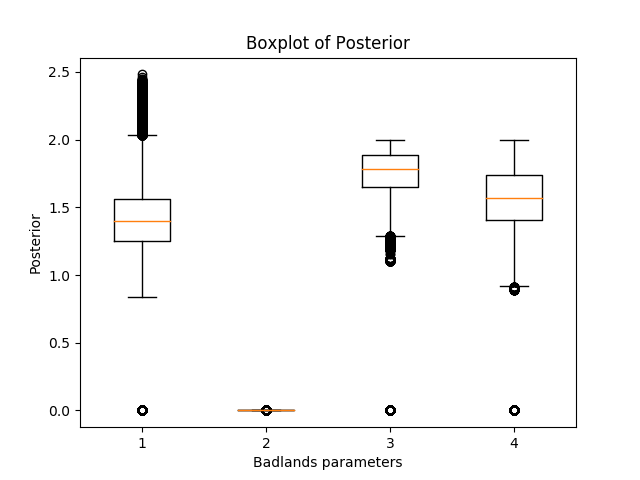
\includegraphics[width=75mm]{crater/badlands_pos.png}}\\
       \subfigure[ eTopo-short posterior  (rainfall, erodibility, m, n, c-aerial, c-marine )]{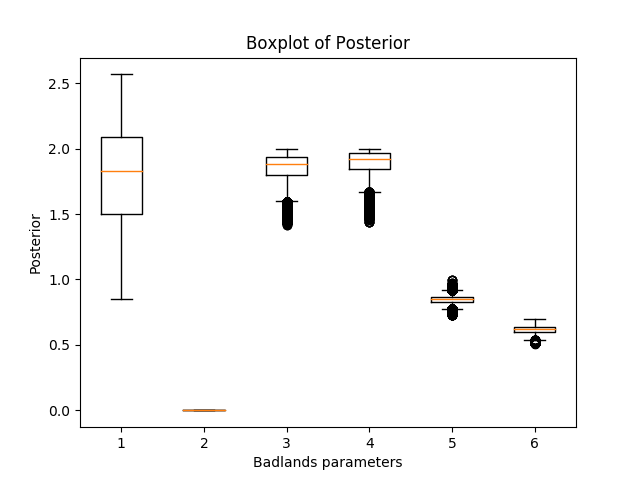
\includegraphics[width=75mm]{etopo_fast/badlands_pos.png}}
      \subfigure[ eTopo posterior  (rainfall, erodibility, m, n, c-aerial, c-marine )]{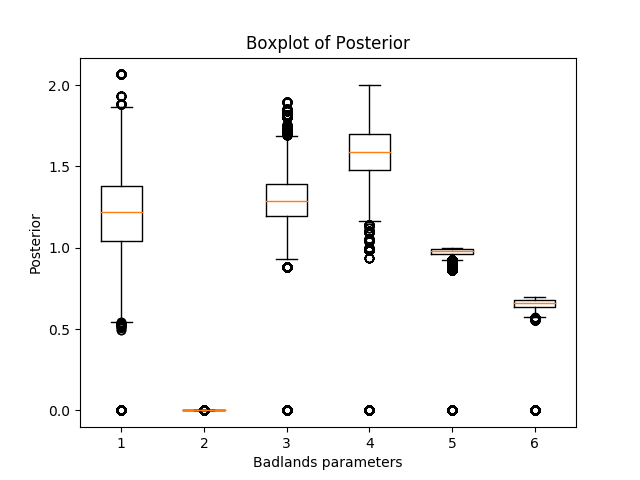
\includegraphics[width=75mm]{etopo/badlands_pos.png}}\\
    \end{tabular}
    \caption{Posterior distribution given as Boxplot   }
 \label{fig:pos_allprob}
  \end{center}
\end{figure*}


\end{document}
